% This is samplepaper.tex, a sample chapter demonstrating the
% LLNCS macro package for Springer Computer Science proceedings;
% Version 2.20 of 2017/10/04
%
\documentclass[runningheads]{llncs}
%
\usepackage{mwe}
\usepackage{graphicx}
\graphicspath{{figures/}}
\usepackage{color}
\definecolor{highlight}{rgb}{1,1,0.6}
\definecolor{link}{rgb}{0.5,0.0,0.0}
\definecolor{cite}{rgb}{0.0,0.0,0.6}
\definecolor{url} {rgb}{0.3,0.0,0.3}
\definecolor{grey}{rgb}{0.3,0.3,0.3}

\usepackage[hidelinks]{hyperref}
\hypersetup{
	colorlinks,
	linkcolor={cite},
	citecolor={cite},
	urlcolor ={cite}
}

\usepackage{tabularx}
\usepackage{array}
\usepackage{booktabs} % for nice rules/lines in tables
\usepackage{arydshln} % for dashed lines in tables

\usepackage{soul} % for highlighting text
\usepackage{xspace}
\usepackage[shortcuts]{extdash}
\usepackage{relsize} % used in the \anote and \comment macros.

%% annotation commands %% 
\newcommand{\anote}[1]{{\leavevmode\smaller\itshape\color{red}\{#1\}}}
\sethlcolor{highlight}
\newcommand{\comment}[2]{\hl{#1} {{\leavevmode\smaller\color{red}\itshape\{#2\}}}}

%% PM Define authornote command for comments
\newcommand{\authornote}[1] {
	\begin{center}
		\framebox{
			{\begin{minipage}[t]{0.9\linewidth}
					\raggedright  \textbf{[PM]}~ \scriptsize #1 \normalsize
			\end{minipage}}
		}
	\end{center}
}

\newcommand*{\bibfont}{\tiny}



\newcommand{\demon}{{DEMON}}
\newcommand{\infomap}{{Infomap}}

\usepackage{amssymb}
\usepackage{bm}
\usepackage{mathtools}

% custom commands
\usepackage{rotating}
\newcolumntype{P}[1]{>{\centering\arraybackslash}p{#1}}
\newcolumntype{Y}{>{\centering\arraybackslash}X}
\usepackage{subcaption}


\begin{document}
    %
    \title{A customisable pipeline for continuously harvesting socially-minded Twitter users}
    %
    \titlerunning{Harvesting socially-minded Twitter users}
    % If the paper title is too long for the running head, you can set
    % an abbreviated paper title here
    %
    \author{Flavio Primo\inst{1} \and
    Paolo Missier\inst{1}\orcidID{0000-0002-0978-2446} \and
    Alexander Romanovsky\inst{1}\orcidID{0000-0002-4076-3331} \and
    Mickael Figueredo\inst{2} \and
    Nelio Cacho\inst{2}}
    
    %
    \authorrunning{F. Primo et al.}
    % First names are abbreviated in the running head.
    % If there are more than two authors, 'et al.' is used.
    %
    \institute{Newcastle University, School of Computing \\
    Science Central, Newcastle upon Tyne, UK \\
    \email{\{firstname.lastname\}@ncl.ac.uk}  \and
    Universidade Federal do Rio Grande do Norte \\
    Natal/RN - Brasil\\
    \email{neliocacho@dimap.ufrn.br}}
    %
    \maketitle       % typeset the header of the contribution
    %
    
    \begin{abstract}
    	On social media platforms and Twitter in particular, specific classes of users such as \textit{influencers}  have been given satisfactory operational definitions in terms of  network and content metrics.
    	Others, for instance \textit{online activists}, are not less important but their characterisation still requires experimenting.
    	%
    	We make  the hypothesis that such interesting users can be found within temporally and spatially localised \textit{contexts}, i.e., small but topical fragments of the network containing interactions about social events or campaigns with a significant footprint on Twitter.
    	To explore this hypothesis, we have designed a continuous user profile discovery pipeline that produces an ever-growing dataset of user profiles by harvesting and analysing contexts from the Twitter stream.
    	The profiles dataset includes key network and content-based users metrics, enabling experimentation with user-defined score functions that characterise specific classes of online users.
        The paper describes the design and implementation of  the pipeline and its empirical evaluation on a case study consisting of healthcare-related campaigns in the UK, showing how it supports experimental operational definitions of online activism. The code is publicly available.
    	
    	\keywords{Twitter analytics \and online user discovery \and online activists \and online influencers \and influence theories}
    \end{abstract}
    %
    
    %\begin{abstract}
    %On social media platforms and Twitter in particular, \textit{influencers} and similar classes of users have been given satisfactory operational definitions in terms of Twitter content metrics.
    %Others, for instance \textit{online activists}, are no less important in practice but have been less precisely defined.
    %Supervised approaches that rely on experts' labelling of users to validate such operational definitions are often questionable, as the labels are typically biased and limited to small validation sets.
    %%
    %In contrast, we suggest a semi-supervised approach that combines two main elements. 
    %Firstly, we identify sets of \textit{contexts}, i.e., small but topical fragments of the network from social events or campaigns that have with a significant footprint on Twitter.
    %We make the hypothesis that such contexts contain meaningful signals to help us recognise activists. 
    %Secondly, we apply network analysis and community detection techniques to identify candidate user profiles within each context, and associate a set of quantitative Twitter-related user metrics to them.
    %As new online contexts occur continuously, this results in an ever-growing, feature-rich dataset of user profiles, which provides an experimental testbed. In our case, we use it to seek ranking functions that correspond to the intuitive notion of online activism.
    %In this paper we describe the design and implementation of the contexts harvesting and dataset population process, and we empirically demonstrate the process in action on a case study consisting of healthcare-related campaigns in the UK, showing how it supports operational definitions of online activism.
    %
    %\keywords{Twitter analytics \and online user discovery \and online activists \and online influencers \and influence theories}
    %\end{abstract}
    %%

    % Sections
    \section{Introduction}

In this paper we present a generic and customisable software framework for incrementally discovering and ranking individual profiles for classes of online users, through analysis of their social activity in micro-blogging platforms, specifically Twitter.
Practical motivation for this work comes from our ongoing effort to support health officers in tropical countries, specifically in Brazil, in their fight against airborne virus epidemics like Dengue and Zika, which are carried by mosquitoes. Help from community activists is badly needed to supplement the scarce public resources deployed on the ground. Our past work has therefore focused on identifying relevant content on Twitter that may point health authorities directly to mosquito breeding sites~\cite{Sousa2018}, as well as to users who have shown interest in those topics, i.e., by posting relevant content on Twitter~\cite{Missier2017}. 

The approach described in this paper generalises those past efforts, by attempting to discover users who demonstrate an inclination \textit{to become engaged in social issues, regardless of the specific topic}.
We refer to this class of users as \textit{activists}.
The rationale for this approach is that activists who manifest themselves online on a range of social initiatives, may be more sensitive to requests for help on specific issues. 
In the paper we experiment with healthcare-related online campaigns in the UK.

To be clear, this work is not about providing a robust definition of online activism, or to demonstrate that online activism translates into actual engagement in the ``real world''.
%
Instead, we acknowledge that the notion of activist is not as well formalised in the literature as that of, for example, \textit{influencers}. 
Thus, we have developed a generic content processing pipeline which can be customised to target specific users contexts. 
The pipeline repeatedly searches for and ranks Twitter user profiles by collecting a rich set of quantifiable network- and content-based user metrics. 
Once targeted to a specific topic, it provides a tool for exploring operational definitions of user roles, including online activism, i.e., by combining the metrics into higher level user features to be used for ranking.

Although the user harvesting pipeline described in the rest of the paper is generally applicable to the analysis of a variety of user profiles, the search for a satisfactory operational definition of online activism 
provides our main motivation. 
%
According to the Cambridge Dictionary, an \textit{activist} is ``A person who believes strongly in political or social change and takes part in activities such as public protests to try to make this happen''.
%
While activism is well-documented, e.g. in the social movement literature~\cite{doi:10.1080/14742830701497277}, and online activism is a well-known phenomenon \cite{IJoC1246}, research has been limited to the study of its broad societal impact. 
In contrast, we are interested in the fine-grained discovery of activists at the level of the single individual, that is, we seek people who feel passionate about a cause or topic, and who take action for it. 
Searching for online activists is a realistic goal, as activists presence in social media is widely acknowledged, and it is also clear that social media facilitates activists communication and organization \cite{Poell2014,Youmans2012}. 
Specific traits that characterise activists include awareness of causes and social topic and the organization of social gatherings and activities, including in emergency situations, by helping organize support efforts and diffusion of useful information.
 
\subsection{Challenges}
 
The challenges posed by the definition of online activism translate into requirements and technical challenges in systematically harvesting candidate users.
%
Firstly, the potentially more subdue nature of activists, relative to influencers, makes it particularly difficult to separate their online footprint from the background noise of general conversations.
Also, interesting activists are by their nature associated to specific topics and manifest their nature in local contexts, for instance as organisers or participants to local events. 
Finally, we expect personal engagement to be sustained over time and across multiple such contexts. 
These observations suggest that the models and algorithms developed for influencers are not immediately applicable, because they mostly operate on global networks, where less prominent users have less of a chance to emerge.
Some topic-sensitive metrics and models have been proposed to measure social influence, for example, \textit{alpha centrality}~\cite{Bonacich2001,Overbey2013} and the \textit{Information Diffusion} model~\cite{Pal2011}. Algorithms based on topic models have also been proposed to account for topic specificity~\cite{Zhao2011b}. However, these approaches are still aimed at measuring influence, not activism, and assume a one-shot discovery process, as opposed to a continuous, incremental approach.

\subsection{Approach}

To address these challenges, the approach we propose involves two strategies. 
Firstly, we identify suitable contexts that are topic-specific and limited both in time and, optionally, also in space, i.e., regional initiatives, events, or campaigns.
We then search for users only within these contexts, using a combination of network and content metrics. 
This follows the intuition that low-key users who produce weak online signal have a better chance to be discovered when the search is localised and then repeated across multiple such contexts.
By \textit{continuously discovering new contexts} and searching for users engaged in those events and campaigns, we hope to incrementally build up a users' dataset where users who appear in multiple contexts are progressively more strongly characterised.
%
Secondly, to allow experimenting with varying technical definitions of \textit{activist}, we collect a number of network-based and content-based user profile features, mostly known from the literature, and make it available for mining. Those features can be combined to generate scores that can be used to experiment with a variety of user rankings.

\subsection{ Contributions}
The paper makes the following specific contributions.
%
Firstly, we propose a data processing pipeline for harvesting Twitter content and user profiles, based on multiple limited contexts. 
The pipeline includes community detection and network analysis algorithms aimed at discovering users within such limited contexts.

Secondly, we have implemented a comprehensive set of content-based metrics that results into an ever-growing database of user profile features, which can then be used for mining purposes. 
User profiles are updated when they are repeatedly found in multiple contexts.

Lastly, for empirical evaluation of our implementation, we demonstrate an operational definition of the activist profile, defined in terms of the features available in the database, by collecting about 3,500 users  across 25 contexts in the domain of healthcare awareness campaigns in the UK during 2018. 
The application of the approach to the specific challenge of combating tropical disease epidemics in Brazil is currently in progress and is not reported in this paper.

\subsection{Related Work}  \label{sec:related}

The closest body of research to this work is concerned with techniques for the discovery of online \textit{influencers}. 
% The characterisation of online activism given in the introduction is substantially different from that of influencers, which have received much attention in the literature.
According to~\cite{Kardara2015}, influencers are \textit{prominent individuals with special characteristics that enable them to	affect a disproportionately large number of their peers with their actions}.
%
A large number of metrics and techniques have been proposed to make this generic definition operational~\cite{RIQUELME2016949}. 
%
These metrics tend to favour high visibility users across global networks, regardless of their actual impact~\cite{Cha2010MeasuringUI}. 
%
In contrast, activists are typically low-key, less prominent users who only emerge from the crowd by signalling high levels of engagement with one or more specific topics, as opposed to being thought-leaders. 
%
While such behaviour can be described  using well-tested metrics~\cite{RIQUELME2016949}, it should also be clear that new ways to combine those metrics are required.

The algorithm proposed in \cite{MATIC2011} aims to identify influencers based on a single topic context, based on relevant social media conversations.
Metrics include number of ``likes'', viewers per months, post frequency and  number of comments per post, as well as the ratio of positive to negative posts.
As some of these metrics are qualitative and difficult to acquire, however, this approach is not easy to automate.

Another approach to ranking topic-specific influencers within specific events appears in  \cite{Kardara2015}, where network dynamics are accounted for in real-time.
Once again however, the result is to discover users who receive much attention, but cannot create a real impact over users inside one topic.

Machine learning is used in~\cite{Biran2012} to analyse posted content and recognise when a user is able to influence another  inside a conversation.
This however requires substantial a priori ground truth, making this approach impracticable in our case. In addition, the need to create a classifier for each topic limits the scalability of the system.

% Some approaches try to extract the content of conversations over topics to understand the ability of a user to be influential within a topic. , a classifier is trained to identify when an user is able to influence another one inside a conversation. However, in this case the necessity of creating labelled data to build a machine learning classifier makes this approach impracticable in our case, which aims to be most practical possible. 
	
% \anote{\cite{Kardara2015} KARDARA:
% 	Here a new ranking algorithm is proposed to find local influencers on Twitter that appear within the context of a specific event being discussed, incorporating the network dynamics as the event evolves with time. 
% 	Local to an event context but focus on user reputation. 
% 	The above techniques all attempt to define influence as
% 	some measurable attribute or observation in the network, such as how many times an original story appears on a website, or how centrally connected a node is within various defined modules within the networks.
% 	The definition used in this work for influence is “who is being listened to the most”.
% 	- this is not who we are looking for.
% 	- one single large event
% 	- no breakdown into communities
% }\\
\anote{FLAVIO: Differently from the majority of the influencer ranking algorithms, in \cite{Schenk2011} a topic-specific influencer ranking is proposed. First it harvests sequentially timed snapshots of the network of users related to a topic. Then it ranks the users based on the number of followers gained and lost in the considered snapshots.}\\

\anote{FLAVIO: In \cite{Bizid:2015:PUD:2808797.2809411} a model for identifying ``prominent users'' regarding a specific topic event in Twitter is presented. Prominent users are defined as those who focus their attention and communication on the aforementioned topic event. Users are described with a real-time computed feature vector among which considers on-topic and off-topic users activity over Twitter. As for~\cite{Biran2012} problems of scalability and adaptability arise as 2 supervised learning methods are used, one to discriminate prominent users from the rest and the other to rank them.}\\
    \section{Contexts and user metrics}

%Two sets of criteria are used to establish relevance.
%Firstly, a context defined by a combination of spatio-temporal and keyword / hashtag constraints to describe the social topics of interest, for instance ``social health care campaigns'' or ``Zika awareness day in Rio de Janeiro''.
%%
%Secondly, a set of metrics are specified to characterise the relevance of user profiles for a specific domain, along with a user-defined function that is specific to user roles, for instance ``activist'', to compose the features into a single value, i.e., a relevance score, which can then be used to rank user profiles both within and across contexts.
%The metrics are meant to capture some operational definition of relevance for specific kinds of user roles. 

The aim of the pipeline is to repeatedly and efficiently discover user profiles from the Twitter post history within user-specified contexts,\footnote{Our plan is to  automate context discovery in the next phase of this work.} and to use the process to grow a database of feature-rich user profiles that can be ranked according to user-defined relevance functions. 
The criteria used to define contexts, profile relevance functions, and associated user relevance thresholds can be configured for specific applications.

\subsection{Contexts and Context networks} \label{sec:contexts}

As mentioned, contexts are meant to identify events or campaigns around social issues, which are characterised by temporal boundaries and by hashtags and/or keyword terms, and optionally also by spatial constraints, i.e., specified using a geographical bounding box.
These are \textit{weak} contexts, because Twitter does not natively support the notion of event or campaign (unlike, for example, Faceboor or Meetup).
We denote the specification of a generic context as 
\begin{equation}
C = ( s, [t_1, t_2], K )
\label{eq:context}
\end{equation}
where $s$ represents the optional spatial constraint, $[t_1, t_2]$ a time interval, and $K = \{ k_1 \dots k_n\}$ is the set of terms used to filter content within the spatio-temporal boundaries.
%
$C$ defines search criteria, which produce a set $P(C)$ of posts when submitted to Twitter.
We only consider two Twitter activities: an \textit{original tweet}, or a \textit{retweet}.
Let $u(p)$ be the user who originated a tweet $p \in P(C)$.
We say that both $p$ and $u(p)$ are \textit{within context} $C$.

We also define the complement $\Tilde{P}(C)$ of $P(C)$ as the set of posts found using the same spatio-temporal constraints, but which do not contain any of the terms in $K$. More precisely, given a context $C'= ( s, [t_1, t_2], \emptyset )$ with no terms constraints, we define $\Tilde{P}(C) = P(C') \setminus P(C)$. 
We refer to these posts, and their respective users, as ``out of context $C$''.

The set of posts $P(C)$ induces a user-user social network graph $G_C = (V,E)$ where $V$ is the set of all users who have authored any $p \in P(C)$: 
$V = \{ u(p) | p \in P(C) \}$, and a weighted directed edge $e = \langle u_1, u_2, w \rangle$ is added to $E$ for each pair of posts $p_1, p_2$ such that $u(p_1) = u_1, u(p_2) = u_2$ and 
either (i) $p_2$ is a retweet of $p_1$, or (ii) $p_1$ contains a mention of $u_2$.
For any such edge, the weight $w$ is a count of such pairs of posts occurring in $P(C)$ for the same pair of users.

\subsection{User relevance metrics}  \label{sec:metrics}

We support a number of metrics that are generally accepted by the community as forming a core, from which many different social user roles are derived~\cite{RIQUELME2016949}. 
We distinguish amongst three types of features, which differ in the way they are computed from the raw Twitter feed:
\begin{description}
	\item[Content-based metrics] that rely solely on content and not on the user-user graph topology. These metrics are defined relative to a topic of interest, i.e., a context;
	\item[Context-independent topological metrics] that encode context-independent, long-lived relationships amongst users, i.e., follower/followee; and 
	\item[Context-specific topological metrics] that encode user relationships that occur specifically within a context.
\end{description}

All metrics are functions of a few core features that can be directly extracted from Twitter posts. 
We start with a set of features that are commonly used in the literature as a baseline.
Given a context $C$ containing user $u$, we define:
%
\begin{align*}
\mathit{R1}(u) &\text{: Number of retweets by $u$, of tweets from other users in C;}\\
\mathit{R2}(u)&\text{: Number of unique users in $C$, who have been retweeted by $u$;}\\
\mathit{R3}(u)&\text{: Number of retweets of $u$'s tweets;}\\
\mathit{R4}(u)&\text{: Number of unique users in $C$ who retweeted $u$'s tweets;}\\
\mathit{P1}(u)&\text{: Number of original posts by $u$ within $C$;}\\
\mathit{P2}(u)&\text{: Number of web links found in original posts by $u$ within $C$;} \\
\mathit{F1}(u)& \text{: Number of followers of $u$;}\\
\mathit{F2}(u)& \text{: Number of followees of $u$}
\end{align*}
%
Note that, given $C$, we can evaluate some of the features above with respect to either $P(C)$ or  $\Tilde{P}(C)$ independently from each other, that is, we can consider an ``on-context'' and an ``off-context'' version of each feature, with the exception of $\mathit{F1}$ and $\mathit{F2}$ which are context-independent.
%
For example, we are going to write $R1_{on}(u)$ to denote the number of context retweets and $R1_{\mathit{off}}(u)$ the number of out-of-context retweets by $u$, i.e., these are retweets that occur within $C$'s spatio-temporal boundaries, but do not contain any of the hashtags or keywords that define $C$.  
%
We similarly qualify all other features.
%
Using these core features, we have implemented the following metrics.

For \textbf{Content-based metrics}, we have:
\begin{align}
\textit{Topical Focus:~\cite{Missier2017}:} ~ \mathit{TF}(u) & =  \frac{\mathit{P1}_{\mathit{on}}(u)}{\mathit{P1}_{\mathit{off}}(u) +1}    \label{eq:TF}\\
\textit{Topical Strength~\cite{Bizid2018}:} ~\mathit{TS}(u) & =	\frac{\mathit{P2}_{\mathit{on}}(u) \cdot \log(\mathit{P2}_{\mathit{on}}(u) + R3_{\mathit{on}} +1 )}{\mathit{P2}_{\mathit{off}}(u) \cdot \log(\mathit{P2}_{\mathit{off}}(u) + R3_{\mathit{off}} +1 ) + 1}   \label{eq:TS} \\
\textit{Topical Attachment~\cite{Bizid:2015,Poell2014}:} ~\mathit{TA}(u) & = \frac{\mathit{P1}_{\mathit{on}}(u) + \mathit{P2}_{\mathit{on}}(u)}{\mathit{P1}_{\mathit{off}}(u) + \mathit{P2}_{\mathit{off}}(u) +1} \label{eq:TA}
\end{align}

We implement one \textbf{Context-independent topological metric} and one \textbf{Context-specific topological metric}, both commonly used, see e.g.~\cite{RIQUELME2016949}:
\begin{align}
\textit{Follower Rank:}  \quad \mathit{FR}(u) = \frac{\mathit{F1}(u)}{\mathit{F1}(u)+\mathit{F2}(u)}   \label{eq:FR}\\
\textit{In-degree centrality:} \quad \mathit{IC}(u) = \frac{\mathit{indegree}(u)}{N-1}  \label{eq:IDC}
\end{align}
where $N$ is the number of nodes in the network induced by $C$.

Note that the metrics we have selected are a superset of those indicated in recent studies on online activism, namely \cite{Lotan2011} and \cite{Poell2014}, and thus support our empirical evaluation, described in Sec.~\ref{sec:evaluation}.

% \anote{Summary of user features if space allows}
    \section{Incremental User Discovery} \label{sec:Pipeline}
	
The content processing pipeline operates iteratively on a set of contexts within a given area of interest, for instance \textit{2018 UK health campaigns}. This set is initialised at the start of the process and then updated at the end of each iteration, in a semi-automated way. 
The user discovery process is therefore potentially open-ended, as long as new contexts can be discovered.
The new contexts are expected to be within the same topic area, but contexts that ``drift'' to new areas of interest are also acceptable. 
Each iteration takes a context $C$  as input, and selects a subset of the users who participate in $C$, using the topogical criteria described below, along with the  set of their features and metrics. 
These users profiles are added to a database, where entries for repeat users are updated according to a user-defined function. 
%
The pipeline structure is described below, where the numbers are with reference to Fig.~\ref{fig:twitterframework}.

\begin{figure*}
	\centering
	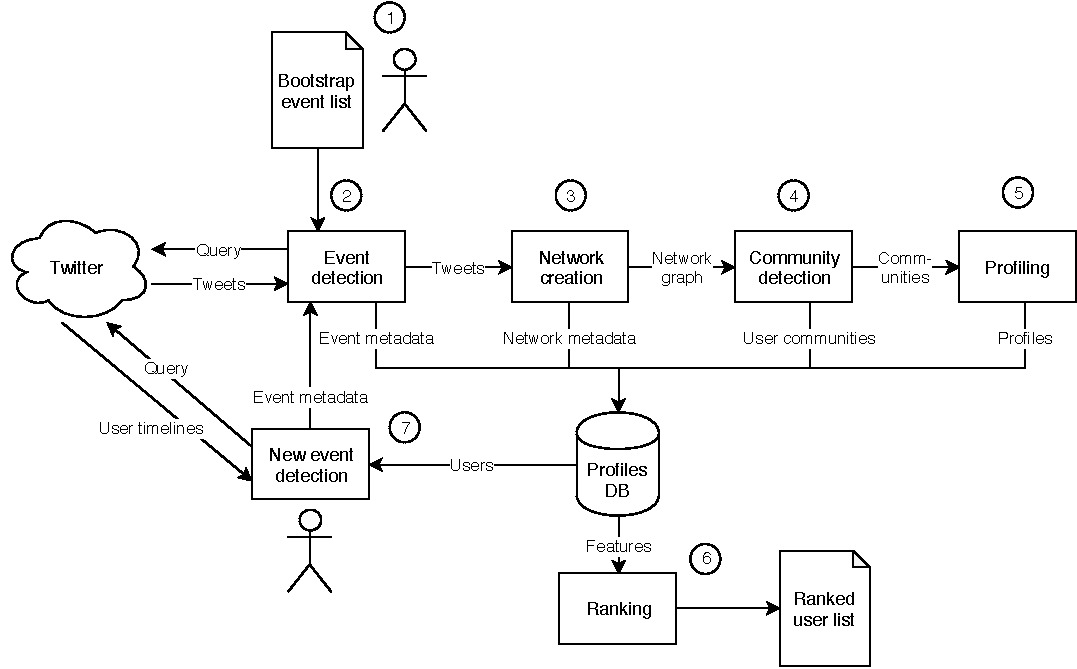
\includegraphics[width=\textwidth]{figures/TwitterFramework}
	\caption{Schematic diagram of the user discovery framework. Note that an initial list $C$ of contexts (events) is provided to initialise the \textit{event detection} step. 
	The outputs from each of these steps are persisted into the Profiles DB.}
	\label{fig:twitterframework}
\end{figure*}

%\subsection{Harvesting Content and Creating Context networks} \label{sec:harvesting}
%
Given $C$ as in (2), all Twitter posts $P(C)$ that satisfy $C$ are retrieved, using the Twitter Search APIs.
Note that this step hits the API service limitations imposed by Twitter. 
For this reason, in our evaluation we have limited our retrieval to 200 tweets/context, which is consistent with our goal to consider many contexts of limited size.
%
The context network $G_C$ is then generated (3), as defined in Sec.~\ref{sec:contexts}.  %To recall, this is a directed network representing retweet and/or mention interactions between pairs of users in $C$. 
The size of each network is largely determined by the nature of the context, and  ranges between 140 and 400 users (avg 254, see Table~\ref{tab:contexts}).

%\subsection{Community detection} \label{sec:communities}

Next, $G_C$  is partitioned into communities of users (4).
The goal of this partitioning is to further narrow the scope when computing in-degree centrality (\ref{eq:IDC}), 
to enable weak-signal users to emerge relative to other more globally dominant users.
%
We have experimented with two of the many algorithms for discovering virtual communities in social networks, namely \demon~\cite{Coscia:2012:DLD:2339530.2339630} and  \infomap~\cite{INFOMAP}. 
Both are available in our implementation, but based on our experimental comparison (Sec.~\ref{sec:evaluation}) we recommend the latter.

\demon~is based on \textit{ego networks}~\cite{Arnaboldi2013}, and uses a label propagation algorithm to assign nodes to communities.  
Users may be assigned to multiple communities, an attractive feature when users are active in more than one community within the same context, i.e., a social event or a campaign.
Label propagation is also a local method, translating into an efficient algorithm.
In practice, however, in our experiments we found that for almost half of our context networks, \demon~actually fails to discover any communities.
%
In contrast, \infomap~forces each user into at most one community, but it generates valid communities in all cases. 
As some of those are very small, our  implementation discards communities with fewer than 4 users (see Sec.~\ref{sec:evaluation}).
%

%
% It has been suggested~\cite{Arnaboldi2013} that ego networks are a useful model not only to describe social relationships amongst people offline, but also the structure of their online connections. 
% Recognising that any individual may have different types of social relationships with different people (i.e., family, friends, colleagues, etc.), \demon~naturally allows for an individual to participate in multiple communities. 

% Specifically, \demon~operates on one node $v$ at a time in our context network $G_C$.

% It applies a \textit{label propagation} algorithm to each neighbour $v'$ of $v$, as follows. First, a new label $l$, which identifies a new community, is tentatively assigned to $v'$. 
% 	Then, with probability $\alpha$ $v'$ changes its label to that of the majority of its own neighbours. 
% 	At this point, each of $v$'s neighbours has a label, which is either new or that of the majority of its own neighbours (except $v$ itself).
% 	$v$ is then assigned majority labels amongst those of its neighbours. 
% 	This determines $v$'s community. 
% 	When more than one label has the same count, $v$ is assigned to all of those communities.
% %
% As a final step, communities that overlap by more than some percentage $\epsilon $ are merged.

Once communities are identified, using either method, we calculate  in-degree centrality (\ref{eq:IDC}) for each node locally, either relative to their own community if they are available, and to the entire network otherwise.

\subsection{Computing user features and ranking} \label{sec:features}


\anote{reviewer comment: 
	
	- In section 3.1, the explanation related to the limitations of the twitter API is not convincing, Specifically, I don’t believe that such limitation is a desired property that allows to “consider many contexts of limited size”. If that is the case, then I would have expected an explanation on how the pipeline (and its configuration) would allow to size a topic according to the API limita
}


Next, user metrics as defined in Sec.~\ref{sec:metrics}, along with the \textit{Follower Rank} are computed from the network and the user features.
%
This is achieved through bulk retrieval of user profile information (5), namely the number of tweets, retweets,  number of followers $F1(u)$ and followees, $F2(u)$, along with user name, web link, and bio.
%
Computing the other metrics: \textit{Topical Focus} (\ref{eq:TF}), \textit{Topical Strength} (\ref{eq:TS}), \textit{Topical Attachment} (\ref{eq:TA}) also requires the entire user post history to be retrieved for the entire time interval defined by the context.
These posts are then separated into $P(C)$ (on-context) and $\Tilde{P}(C)$ (off-context), depending on whether they contain a hashtag related to the context or not.
Similarly, a post that contains a link is a \textit{link on-topic} if it contains both a link and a hashtag related to the context, and a \textit{link off-topic} otherwise.
We also calculate the number of retweets for every post, i.e., $\mathit{R1}(u)$ and $\mathit{R3}(u)$, which are required to compute \textit{Topical Strength}.

All of these features are persisted to a database which is made available for ranking purposes.
User-defined functions can be specified to update the Rank of pre-existing users, e.g. by combining scores assigned at different times.
%
The DB enables user-defined scoring functions, which result in user ranking lists (6). Examples of these are given later in Sec.~\ref{sec:evaluation}.
This framework approach is consistent with the experimental nature of our search for \textit{activists}, which requires exploring a variety of ranking functions.

\subsection{New contexts discovery} \label{sec:context-discovery}

The final step within one iteration (7) aims to discover new contexts, so that the process can start again (2).
Intuitively, once a score function has been applied and users have been ranked, we can hope to discover new interesting keywords and hashtags by exploring the timeline of the top-$k$ users.
Specifically,  we consider each hashtag found in the timelines, which is related to the broader topic and not yet considered in past iterations.
Each stored hashtag is then enriched with the information needed to perform a new iteration of the pipeline, namely (i) the temporal and spatial information of the context, and (ii) related hashtags.
%
Currently this step is only semi-automated, as making a judgement on the relevance of the new terms requires  human expertise.
While automating this step is not straightforward, this is not a very time-consuming step, and one can imagine an approach where such task is crowdsourced.

While the process ends naturally when no new contexts are uncovered from the previous ones, the system continuously monitors the Twitter stream for recent contexts. These may typically include events that are temporally recurring, and use similar hashtags for each new edition. In this case, their relevance is assessed on the basis of their past history.
    \section{Empirical Evaluation} \label{sec:evaluation}

Existing methods to discover specific classes on online users are typically validated using a supervised approach, i.e., they rely on expert-generated ground truth.
Such approaches, however, are vulnerable to the subjectivity of the experts, whereby the evaluation would be measuring the fit of the model to the specific experts' own assessment of user instances' relevance. 
In contrast, we follow an unsupervised approach with no a priori knowledge of user relevance. We aim to demonstrate the value of our pipeline in creating a database of online profiles that are ready to be mined, along with examples of candidate user ranking functions.
In this approach, human expertise only comes into play to assess and validate the top-$k$ user lists produced by these functions.
%
We  demonstrate the pipeline in action on a significant set of 25 initial contexts, and define two alternative ranking functions aimed at capturing the empirical notion of  \textit{online activists}.
%
The pipeline is fully implemented in Python using Pandas and public libraries (NetworkX, Selenium) and is available on github\footnote{ \url{https://github.com/flaprimo/twitter-network-analysis}}. 
All experiments are performed on a single Azure node with standard commodity configuration.
Note that we do not focus on system performance as all components operate in near-real time. One exception is  Twitter content harvesting, which is limited by the Twitter API and requires approximately 2 hours per context.

\subsection{Contexts and networks} \label{sec:contexts-selection}
 
We have manually selected 25 contexts within the scope of health awareness campaigns in the UK, all occurring in 2018 and well-characterised using predefined hashtags.
Due to limitations imposed by Twitter on the number of posts that can be retrieved within a time interval, only $200$ tweets were retrieved from each context.
 Table~\ref{tab:contexts} lists the events along with key metrics for their corresponding user-user networks. 
To recall, \textit{assortativity} measures how frequently nodes are likely to connect to other nodes with the same degree ($>0$) or with a different degree ($<0$). 
Negative figures (mean: -0.22, std dev: 0.17) are in line with what is observed on the broader Twitter network~\cite{Fisher2017}.
%
The very small figures for density, defined as $\frac{\#edges }{\mathit{\mathit{\#nodes}} \cdot (\mathit{\#nodes} -1)}$ (mean: 0.004, std dev: 0.002), suggest very few connections exist amongst users within a context. 
This makes it difficult to detect meaningful communities, as described below, thus for some contexts the topological metrics are measured on the entire network as opposed to within each community.
This view is also supported by the average node degree (mean: 2.04, std dev: 0.46) and the ratio of strongly connected components to the number of nodes (mean: 0.98, std. dev. 0.02).

\begin{table}
	\tiny
	\resizebox{\textwidth}{!}{
	    \begin{tabularx}{\textwidth}{|X|P{2.2cm}|P{1.2cm}|P{1cm}|P{1.4cm}|P{1.2cm}|P{1.3cm}|}

\hline
\textbf{Context name} & \textbf{Period (2018)} & \textbf{Nodes} & \textbf{Edges} & \textbf{Density} & \textbf{Avg degree} & \textbf{Assor-tativity} \\ \hline
16 days of action & 11-25 / 12-10 & 396 & 349 & 0.002 & 1.8 & -0.1 \\ \hline
Elf day & 12-03 / 12-12 & 365 & 436 & 0.003 & 2.4 & -0.2 \\ \hline
Dry january & 01-01 / 01-31 & 235 & 234 & 0.004 & 2.0 & -0.3 \\ \hline
Cervical cancer prevention week & 01-21 / 01-27 & 209 & 192 & 0.004 & 1.8 & -0.1 \\ \hline
Time to talk day & 02-06 / 02-07 & 268 & 231 & 0.003 & 1.7 & -0.2 \\ \hline
Eating disorder awareness week & 02-25 / 03-03 & 256 & 241 & 0.004 & 1.9 & -0.2 \\ \hline
Rare disease day & 02-28 / 03-01 & 294 & 206 & 0.002 & 1.4 & -0.2 \\ \hline
Ovarian cancer awareness month & 03-01 / 03-31 & 215 & 202 & 0.004 & 1.9 & -0.4 \\ \hline
Nutrition and hydration week & 03-11 / 03-17 & 273 & 326 & 0.004 & 2.4 & -0.3 \\ \hline
Brain awareness week & 03-11 / 03-17 & 307 & 281 & 0.003 & 1.8 & -0.1 \\ \hline
No smoking day & 03-13 / 03-14 & 254 & 219 & 0.003 & 1.7 & -0.3 \\ \hline
Epilepsy awareness purple day & 03-26 / 03-27 & 306 & 252 & 0.003 & 1.6 & -0.2 \\ \hline
Experience of care week & 04-23 / 04-27 & 176 & 196 & 0.006 & 2.2 & -0.1 \\ \hline
Brain injury week & 05-01 / 05-31 & 238 & 306 & 0.005 & 2.6 & -0.1 \\ \hline
Mental health awareness week & 05-14 / 05-20 & 268 & 245 & 0.003 & 1.8 & -0.5 \\ \hline
Dementia action week & 05-21 / 05-31 & 300 & 300 & 0.003 & 2.0 & -0.0 \\ \hline
Mnd awareness month & 06-01 / 06-30 & 141 & 234 & 0.012 & 3.3 & -0.3 \\ \hline
Wear purple for jia & 06-01 / 06-30 & 165 & 245 & 0.009 & 3.0 & -0.5 \\ \hline
Carers week & 06-11 / 06-17 & 270 & 277 & 0.004 & 2.1 & 0.0 \\ \hline
National dementia carers & 09-09 / 09-10 & 184 & 177 & 0.005 & 1.9 & -0.2 \\ \hline
Mens health week & 06-11 / 06-17 & 264 & 214 & 0.003 & 1.6 & -0.2 \\ \hline
Stress awareness day & 11-07 / 11-08 & 293 & 209 & 0.002 & 1.4 & -0.2 \\ \hline
National dyslexia week & 10-01 / 10-07 & 229 & 235 & 0.004 & 2.1 & -0.2 \\ \hline
Ocd awareness week & 10-07 / 10-13 & 202 & 193 & 0.005 & 1.9 & -0.6 \\ \hline
Jeans for genes day & 09-21 / 09-22 & 246 & 325 & 0.005 & 2.6 & -0.2 \\ \hline

\end{tabularx}

	}
	\caption{List of contexts used in the experiments along with network metrics.}
	\label{tab:contexts}
\vspace{-20pt}
\end{table}


\subsection{Communities}  \label{sec:communities-eval}

 \demon~and \infomap~ produce significantly different communities in each network. 
%
\demon~identifies communities in only 48\% of the networks, with an average of only 1.92 communities per network and 
a slightly negative  (-0.28) average assortativity  per community, in line with the average for their parent networks.
%
Only the users who belong to one of those communities, about 6\%, are added to the database.
%
For the remaining 52\% of networks where no communities are detected, users' in-degrees are calculated using the entire network, and all users are added to the database, 
for a total of 3,570 users being added to the database in our experiments using \demon.

In contrast, \infomap~provides meaningful communities for all networks.
Those with fewer than 3 users are discarded, leaving  18.88 communities per network on average, with 8.5 users per community on average.
% The rightmost column in Table~\ref{tab:contexts} reports the number of communities normalised by the size of the network, where a  contains . 
When using Infomap, 3,567 users were added to the database (on average 253 users per network).
The average assortativity across all communities is again slightly negative (-0.43).
%
Table~\ref{tab:demon-vs-infomap} compares the two approaches on the key metrics just discussed. On the basis of this comparison, we recommend using \infomap, which we have used for  our evaluation.

\begin{table}
	\vspace{-10pt}
		\footnotesize
	\resizebox{\textwidth}{!}{
	    \begin{tabularx}{\textwidth}{|X|P{1.7cm}|P{1.7cm}|}
\hline
\textbf{Metric} & \textbf{\demon} & \textbf{\infomap} \\ \hline
Fraction of networks with null communities & 0.52 & 0.0 \\ \hline
Number of communities per context (avg) & 1.92 & 18.88 \\ \hline
Fraction of network users added to the DB  (avg) & 0.06 & 0.59 \\ \hline
Fraction of repeat users  added to the DB across networks & 0.28 & 0.37 \\ \hline
\end{tabularx}
	}
	\caption{Comparing \demon~to \infomap~for community detection.}
	\label{tab:demon-vs-infomap}
	\vspace{-20pt}
\end{table}

\subsection{Users discovery}  \label{sec:users}

Repeat users who appear in multiple contexts are particularly interesting as they provide a stronger signal. 
Out of the total 3,567 users, 160 of those appear at least in two of the 25 contexts.
After community detection, only 61 of these users are still seen as repeat users,
while the remaining 99 are either removed altogether, or they only appear once.
Of the 61, 57 appear twice, 2 appear three times, and 2 appear four times. 
Thus, only 1.6\% of users appear more than once when communities with more than 3 users are considered, compared to the overall 4.5\% of overall repeat users.
%
Table~\ref{tab:repeat-users} reports the top-10 repeat users along with their \textit{Follower Rank}, and Fig.~\ref{fig:repeat-users-frequency} shows the number of repeat users per context.
As the table is sorted by number of occurrences then by \textit{Follower Rank}, an indication of popularity,  it is not surprising to find that top users include well-known names such as Mr. Hunt, who at the time of the events was Secretary of State for Health and Social Care in the UK, with $FR =1$, and a number of associations and foundations active in the public healthcare space.
More interesting are perhaps non-repeat users who emerge when ad hoc ranking is applied to the database, as we illustrate next.

\begin{table}[htb]
	\centering
	\footnotesize
	\resizebox{\textwidth}{!}{
		\begin{tabularx}{\textwidth}{|p{2.5cm}|X|P{2.4cm}|P{2.4cm}|}
\hline
\textbf{Username} & \textbf{Name} & \textbf{Follower rank} & \textbf{Participations} \\ \hline
alzheimerssoc & Alzheimer's Society & 0.99 & 4 \\ \hline
dementiauk & Dementia UK & 0.98 & 4 \\ \hline
mentalhealth & Mental Health Fdn & 0.97 & 3 \\ \hline
colesmillerllp & Coles Miller LLP & 0.65 & 3 \\ \hline
rdash\_nhs & RDaSH NHS FT & 0.88 & 2 \\ \hline
alzsocseengland & Alzheimer's Society - South ... & 0.64 & 2 \\ \hline
jeremy\_hunt & Jeremy Hunt & 1.0 & 2 \\ \hline
nhsengland & NHS England & 0.99 & 2 \\ \hline
carersuk & Carers UK & 0.95 & 2 \\ \hline
mndassoc & MND Association & 0.64 & 2 \\ \hline
\end{tabularx}
	}
	\caption{Top-10 repeat users, amongst those who belong to a community.}
	\label{tab:repeat-users}
	\vspace{-20pt}
\end{table}

\begin{figure*}[htb]
	\centering
	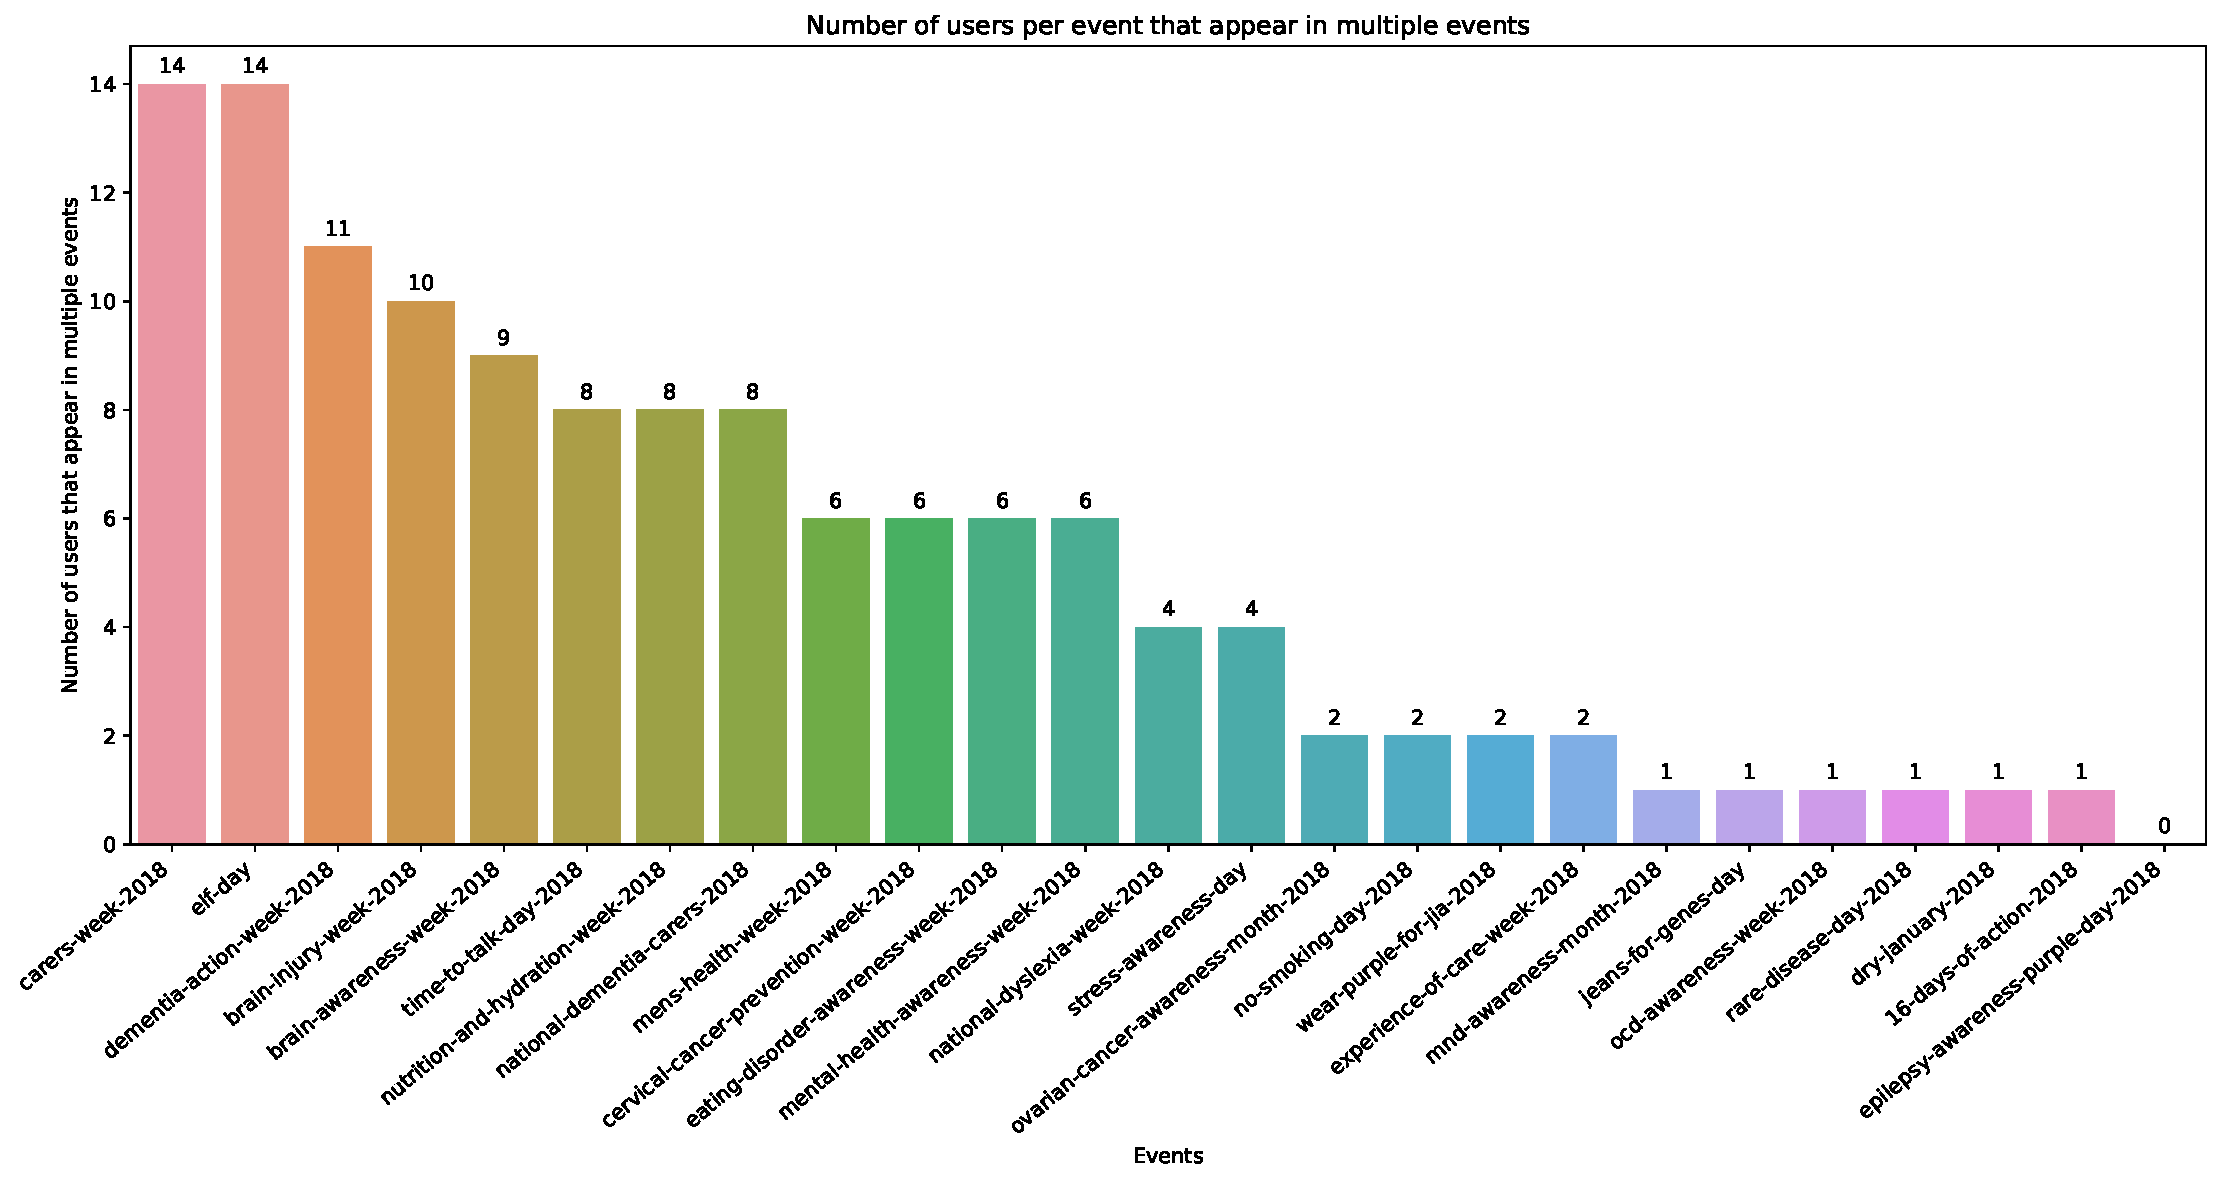
\includegraphics[width=1.2\textwidth]{figures/repeat-users-frequency}
	\caption{Number of repeat users for each context}
	\label{fig:repeat-users-frequency}
\end{figure*}

\vspace{-10pt}
\subsection{Users ranking} \label{sec:ranking}
%\vspace{-10pt}

To demonstrate the potential value of the database, albeit on a small scale, we have tested two user ranking functions.
As mentioned, the aim of this exercise is to provide an objective grounding for engaging with experts on finding suitable operational definitions for specific user profiles.
%
\begin{table}
			\vspace{-20pt}
	\centering
	\footnotesize
	\resizebox{\textwidth}{!}{
		% \begin{tabular}{P{0.6cm}|p{2.3cm}|P{1.4cm}|P{1.8cm}|p{2.3cm}|P{1.4cm}|P{1.8cm}|}

% \cline{2-7}
% \multicolumn{1}{l|}{} & \multicolumn{3}{c|}{\textbf{Ranking 1}} & \multicolumn{3}{c|}{\textbf{Ranking 2}} \\ \hline
% \multicolumn{1}{|c|}{\textbf{\#}} & \textbf{User} & \textbf{On-topic} & \textbf{Individual} & \textbf{User} & \textbf{On-topic} & \textbf{Individual} \\ \hline
% \multicolumn{1}{|c|}{1} & homesnutrition & X &  & johnneustadt & X & X \\ \hline
% \multicolumn{1}{|c|}{2} & ficajones & X & X & jo\_millar27 & X & X \\ \hline
% \multicolumn{1}{|c|}{3} & helenvweaver & X & X & hatchbrenner &  &  \\ \hline
% \multicolumn{1}{|c|}{4} & spriggsnutri & X &  & nchawkes & X & X \\ \hline
% \multicolumn{1}{|c|}{5} & critcarelthtr & X &  & moz0373runner & X & X \\ \hline
% \multicolumn{1}{|c|}{6} & danielleroisin\_ & X & X & aimsonhealth & X & X \\ \hline
% \multicolumn{1}{|c|}{7} & mynameisandyj & X & X & wordsharkv5 &  & X \\ \hline
% \multicolumn{1}{|c|}{8} & fionaliu92 & X & X & fullcircle\_play & X &  \\ \hline
% \multicolumn{1}{|c|}{9} & ldpartnership & X &  & qsprivatehealth & X &  \\ \hline
% \multicolumn{1}{|c|}{10} & milaestevam1 &  & X & socialissp &  &  \\ \hline

% \end{tabular}

\begin{tabular}{P{0.6cm}|p{2.3cm}|P{1.4cm}|P{1.8cm}|p{2.3cm}|P{1.4cm}|P{1.8cm}|p{2.3cm}|P{1.4cm}|P{1.8cm}|}

\cline{2-10}
\multicolumn{1}{l|}{} & \multicolumn{3}{c|}{\textbf{Ranking 1}} & \multicolumn{3}{c|}{\textbf{Ranking 2}} & \multicolumn{3}{c|}{\textbf{Ranking 3}} \\ \hline
\multicolumn{1}{|c|}{\#} & \textbf{User} & \textbf{On-topic} & \textbf{Individual} & \textbf{User} & \textbf{On-topic} & \textbf{Individual} & \textbf{User} & \textbf{On-topic} & \textbf{Individual} \\ \hline
\multicolumn{1}{|c|}{1} & homesnutrition & X &  & johnneustadt & X & X & johnneustadt &  & X \\ \hline
\multicolumn{1}{|c|}{2} & ficajones & X & X & jo\_millar27 & X & X & solutions777 & X & X \\ \hline
\multicolumn{1}{|c|}{3} & helenvweaver & X & X & hatchbrenner &  &  & kingste29344921 & X & X \\ \hline
\multicolumn{1}{|c|}{4} & spriggsnutri & X &  & nchawkes & X & X & daisylu1964 & X &  \\ \hline
\multicolumn{1}{|c|}{5} & critcarelthtr & X &  & moz0373runner & X & X & zakariamarsli & X & X \\ \hline
\multicolumn{1}{|c|}{6} & danielleroisin\_ & X & X & aimsonhealth & X & X & meowaaaaaa & X &  \\ \hline
\multicolumn{1}{|c|}{7} & mynameisandyj & X & X & wordsharkv5 &  & X & vecta67 & X &  \\ \hline
\multicolumn{1}{|c|}{8} & fionaliu92 & X & X & fullcircle\_play & X &  & cosfordfamily1 & X & X \\ \hline
\multicolumn{1}{|c|}{9} & ldpartnership & X &  & qsprivatehealth & X &  & hayleycorriganx & X &  \\ \hline
\multicolumn{1}{|c|}{10} & milaestevam1 &  & X & socialissp &  &  & jhbrasfie & X &  \\ \hline

\end{tabular}
	}
	\caption{Top-10 ranked users for ranking functions (\ref{eq:rank1}) and (\ref{eq:rank2}), with indication of whether the user is on-topic/off-topic and individual vs association.}
	\label{tab:rank1}
	\vspace{-30pt}
\end{table}
%

\begin{align}
\textit{Ranking 1:} ~ \mathit{R1}(u) & = \frac{1}{\sum_{u \in C} \mathit{IC}(u) + 1} \cdot \sum_{u \in C} \mathit{TF}(u) \label{eq:rank1} \\
\textit{Ranking 2:} ~ \mathit{R2}(u) & = \lvert \mathit{FR}(u) - 1 \rvert \cdot \left(\sum_{u \in C} \mathit{TA}(U) + \sum_{u \in C} \mathit{IC}(U)\right) \label{eq:rank2} \\
\textit{Ranking 3:} ~ \mathit{R3}(u) & = \lvert \mathit{FR}(u) - 1 \rvert \cdot \left(\sum_{u \in C} \mathit{TA}(U) + \frac{1}{\sum_{u \in C} \mathit{IC}(U) + 1}\right) \label{eq:rank3}
\end{align}
%
Function (\ref{eq:rank1}) is designed to promote users who are at the ``fringe'' of their community, while giving credit to generic on-topic activities during the contexts. 
To achieve this, \textit{Topical Focus} $\mathit{TF}$ is used as a positive contribution, while a large in-degree $\mathit{IC}$ reduces the score.
%
In contrast, function (\ref{eq:rank2}) penalises user popularity, i.e., by using the complement of \textit{Follower Rank} $\mathit{FR}$, while rewarding prominence inside communities (in-degree $\mathit{IC}$) and information spreading by also considering shared links (\textit{Topical Attachment} $\mathit{TA}$).

The top-10 users for each ranking are reported in Tab.~\ref{tab:rank1}. To appreciate of the effects of these functions, we have manually labelled the top-100 user profiles for each of the rankings, using a broad type classification as \textit{individual} as opposed to \textit{institutional players} (associations, public bodies), or \textit{professionals}. 
Our results show that  (\ref{eq:rank1}) seems to favour more on-topic users (90\% for  (\ref{eq:rank1})  vs 70\% for  (\ref{eq:rank2})), 
while  (\ref{eq:rank2}) favours more individuals (55\% for (\ref{eq:rank1})  and 71\% for (\ref{eq:rank2})), among in-topic users.
%
Both functions rank on-topic users highly (90\% for (\ref{eq:rank1}) and 70\% for (\ref{eq:rank2})).
Also, repeat users are rewarded in both rankings. Users with $\mathit{FR}(u) = 0$ and $\mathit{min\_max(\lvert Tweets (u)\rvert) < 0.005}$ are considered not active and have been assigned lowest score.
Fig.~\ref{fig:ranks-distribution} shows the distribution of user types within the top-100 users for each of the two rankings, broken down into 10 users bins. We can see that individuals are 33\% in each case, but they tend to emerge earlier in the ranks when (\ref{eq:rank2}) is used.
We plan to conduct user studies to establish useful analytics to be incorporated into our framework. 
\begin{figure}
	\centering
	\begin{subfigure}{.49\textwidth}
		\centering
		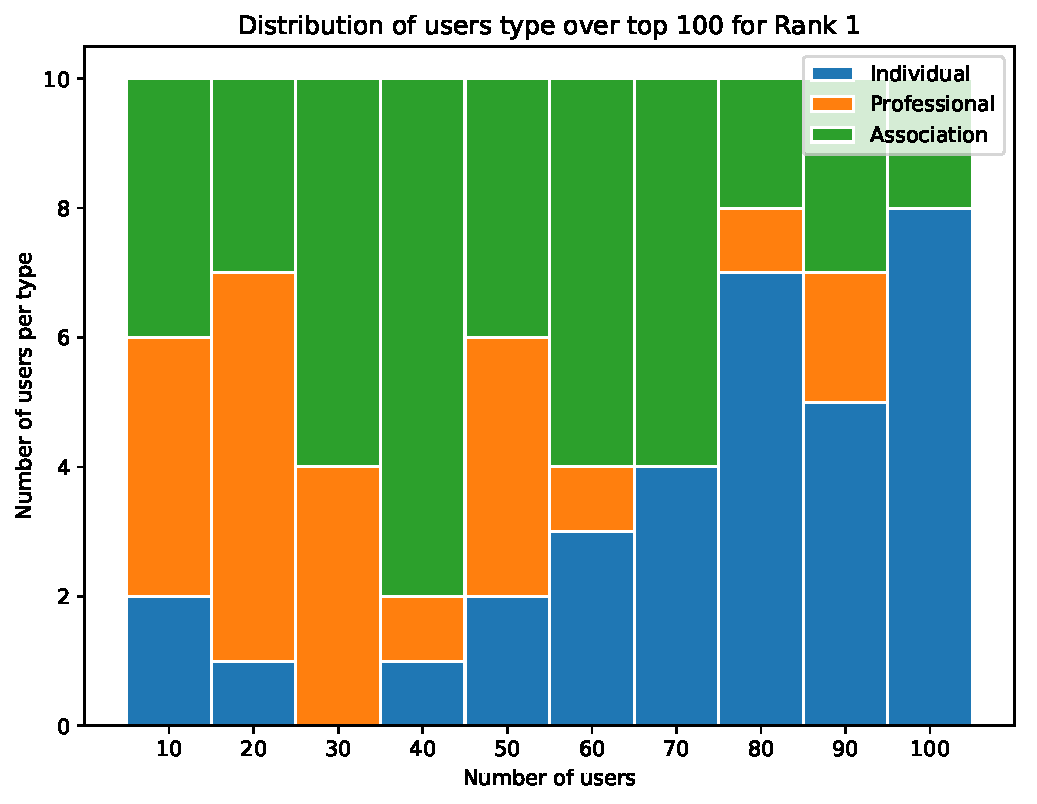
\includegraphics[width=\textwidth]{figures/rank1-distribution.pdf}
		\caption{Rank 1: 33 are individuals, 23 are professionals, 44 are associations}
		\label{fig:rank1-distribution}
	\end{subfigure}
	\hfill%
	\begin{subfigure}{.49\textwidth}
		\centering
		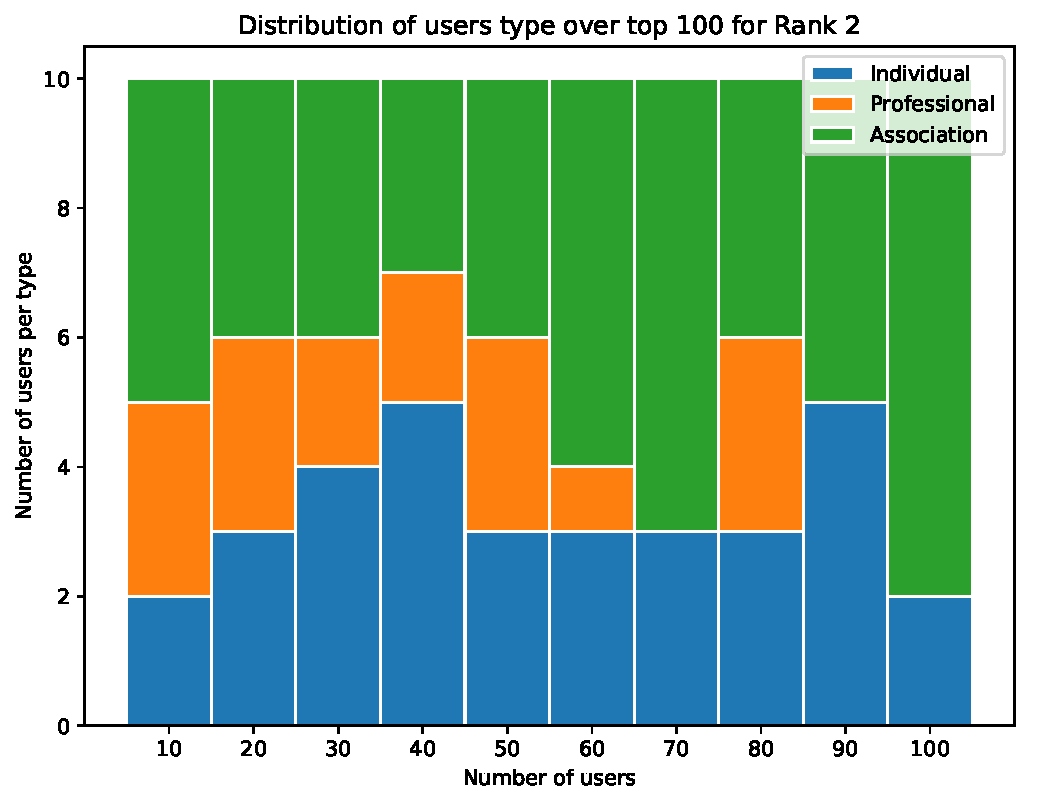
\includegraphics[width=1\textwidth]{figures/rank2-distribution.pdf}
		\caption{Rank 2: 33 are individuals, 17 are professionals, 50 are associations}
		\label{fig:rank2-distribution}
	\end{subfigure}
	\hfill%
	\begin{subfigure}{.49\textwidth}
		\centering
		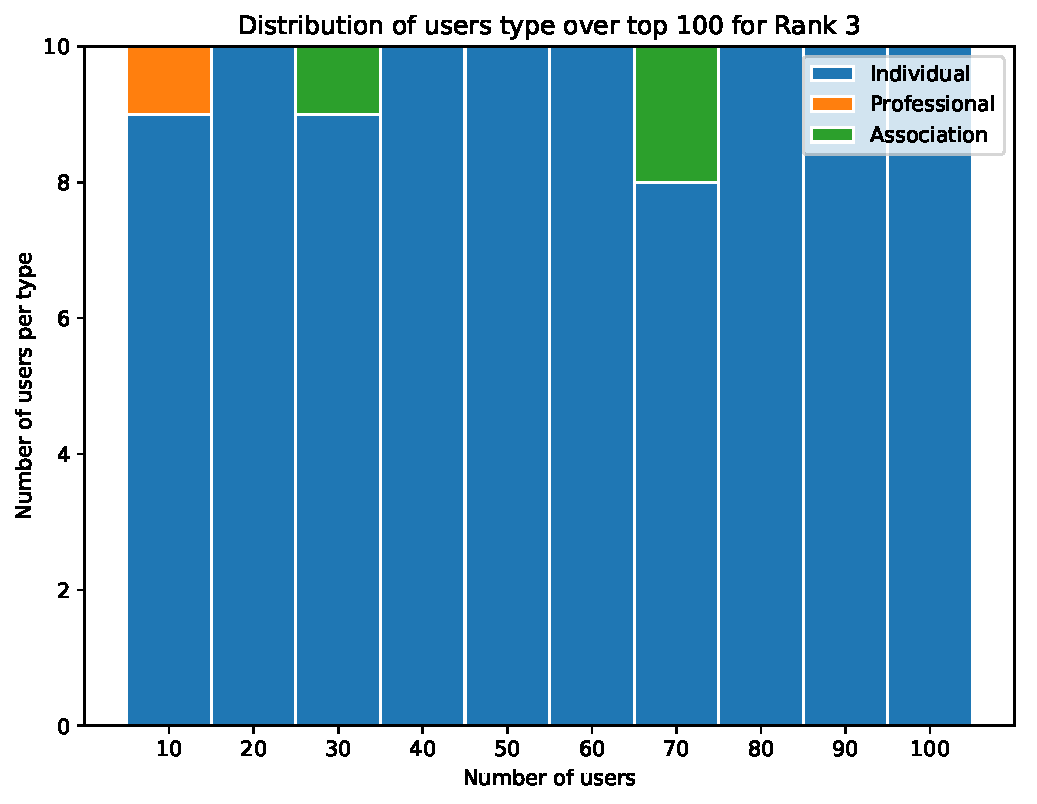
\includegraphics[width=1\textwidth]{figures/rank3-distribution.pdf}
		\caption{Rank 3: 96 are individuals, 1 are professionals, 3 are associations}
		\label{fig:rank3-distribution}
	\end{subfigure}
	\caption{Top 100 user type distribution for the ranks.}
	\label{fig:ranks-distribution}
\end{figure}
%
    \vspace{-10pt}
\section{Conclusions and lessons learnt}
\vspace{-10pt}


Motivated by the need to find an operational definition of ``online activists'' that is grounded in well-established network and user-activity metrics, we have designed a Twitter content processing pipeline for systematically harvesting Twitter users based on their engagement with online socially-minded events, or campaigns, which we have called \textit{contexts}.
The pipeline yields an incrasingly growing database of user profiles along with a number of metrics, which can then be analysed to experiment with user-defined user ranking criteria. The structure and the components of the pipeline are designed to pre-select promising candidate profiles, but the approach is unsupervised, i.e., no manual classification of example users is provided.
We have empirically evaluated the pipeline on a case study, along with experimental scoring functions to show the viability of the approach. 

\anote{add if space permits:
	
	However, I miss a fundamental “lesson learned”section: what did you learn in the design, development, and testing of your pipeline, that could be of interest for other scientists and practitioners? The current evaluation is useful in showing some properties of the pipeline, but it does not provide relevant insights beyond the experience acquired in the use case,
	
}

We are currently experimenting with ideas for automating the discovery of new contexts so that the pipeline may continuously add new users to the database, and update its metrics for an increasing number of  repeat users.

%    \bibliographystyle{splncs04}
%    \bibliography{icwe19}

\footnotesize
% This is samplepaper.tex, a sample chapter demonstrating the
% LLNCS macro package for Springer Computer Science proceedings;
% Version 2.20 of 2017/10/04
%
\documentclass[runningheads]{llncs}
%
\usepackage{mwe}
\usepackage{graphicx}
\graphicspath{{figures/}}
\usepackage{color}
\definecolor{highlight}{rgb}{1,1,0.6}
\definecolor{link}{rgb}{0.5,0.0,0.0}
\definecolor{cite}{rgb}{0.0,0.0,0.6}
\definecolor{url} {rgb}{0.3,0.0,0.3}
\definecolor{grey}{rgb}{0.3,0.3,0.3}

\usepackage[hidelinks]{hyperref}
\hypersetup{
	colorlinks,
	linkcolor={cite},
	citecolor={cite},
	urlcolor ={cite}
}

\usepackage{tabularx}
\usepackage{array}
\usepackage{booktabs} % for nice rules/lines in tables
\usepackage{arydshln} % for dashed lines in tables

\usepackage{soul} % for highlighting text
\usepackage{xspace}
\usepackage[shortcuts]{extdash}
\usepackage{relsize} % used in the \anote and \comment macros.

%% annotation commands %% 
\newcommand{\anote}[1]{{\leavevmode\smaller\itshape\color{red}\{#1\}}}
\sethlcolor{highlight}
\newcommand{\comment}[2]{\hl{#1} {{\leavevmode\smaller\color{red}\itshape\{#2\}}}}

%% PM Define authornote command for comments
\newcommand{\authornote}[1] {
	\begin{center}
		\framebox{
			{\begin{minipage}[t]{0.9\linewidth}
					\raggedright  \textbf{[PM]}~ \scriptsize #1 \normalsize
			\end{minipage}}
		}
	\end{center}
}

\newcommand*{\bibfont}{\tiny}



\newcommand{\demon}{{DEMON}}
\newcommand{\infomap}{{Infomap}}

\usepackage{amssymb}
\usepackage{bm}
\usepackage{mathtools}

% custom commands
\usepackage{rotating}
\newcolumntype{P}[1]{>{\centering\arraybackslash}p{#1}}
\newcolumntype{Y}{>{\centering\arraybackslash}X}
\usepackage{subcaption}


\begin{document}
%
\title{Fantastic activists and how to find them\thanks{} \\ \small (not the real title)}
%
%\titlerunning{Abbreviated paper title}
% If the paper title is too long for the running head, you can set
% an abbreviated paper title here
%
\author{Flavio Primo\inst{1} \and
Paolo Missier\inst{1}\orcidID{0000-0002-0978-2446} \and
Alexander Romanovsky\inst{1} \and
Mickael Figueredo\inst{2} \and
Nelio Azevedo Cacho\inst{2}}

%
\authorrunning{F. Primo et al.}
% First names are abbreviated in the running head.
% If there are more than two authors, 'et al.' is used.
%
\institute{Newcastle University, School of Computing Science \\
Science Central, Newcastle upon Tyne, UK \\
\email{\{firstname.lastname\}@ncl.ac.uk}  \and
Universidade Federal do Rio Grande do Norte \\
Natal/RN - Brasil\\
\email{neliocacho@dimap.ufrn.br}}
%
\maketitle       % typeset the header of the contribution
%
\begin{abstract}
On social media platforms and Twitter in particular, \textit{influencers}c and other classes of users have been given satisfactory operational definitions in terms of Twitter content metrics.
Others, for instance \textit{online activists}, are no less important in practice but have been less precisely defined.
Supervised approaches that rely on experts' labelling of users to validate such operational definitions are often questionable, as the labels are typically biased and limited to small validation sets.
%
In contrast, we suggest a semi-supervised approach that combines two main elements. 
Firstly, we identify sets of \textit{contexts}, i.e., small but topical fragments of the  network from social events or campaigns that have with a significant footprint on Twitter.
We make the hypothesis that such context contain meaningful signals to help us recognise activists. 
Secondly, we apply network analysis and community detection techniques to identify candidate user profiles within each context,  and we associate a set of quantitative Twitter-related user metrics to them.
As new online contexts occur continuously, this results in an ever-growing, feature-rich dataset of user profiles, which provides an experimental testbed. In our case, we use it to seek ranking functions that correspond to the intuitive notion of online activism.
In this paper we describe the design and implementation of the contexts harvesting and dataset population process, and we empirically demonstrate the process in action on a case study consisting of healthcare-related campaigns in the UK, showing how it supports operational definitions of online activism.

\keywords{Twitter analytics \and online user discovery \and online activists \and online influencers \and influence theories}
\end{abstract}
%

\section{Introduction}

In this paper we present a generic and customisable software framework for incrementally discovering and ranking individual profiles for classes of online users, through analysis of their social activity in micro-blogging platforms, specifically Twitter.
Practical motivation for this work comes from our ongoing effort to support health officers in tropical countries, specifically in Brazil, in their fight against airborne virus epidemics like Dengue and Zika, which are carried by mosquitoes. Help from community activists is badly needed to supplement the scarce public resources deployed on the ground. Our past work has therefore focused on identifying relevant content on Twitter that may point health authorities directly to mosquito breeding sites~\cite{Sousa2018}, as well as to users who have shown interest in those topics, i.e., by posting relevant content on Twitter~\cite{Missier2017}. 

The approach described in this paper generalises those past efforts, by attempting to discover users who demonstrate an inclination \textit{to become engaged in social issues, regardless of the specific topic}.
We refer to this class of users as \textit{activists}.
The rationale for this approach is that activists who manifest themselves online on a range of social initiatives, may be more sensitive to requests for help on specific issues. 
In the paper we experiment with healthcare-related online campaigns in the UK.

To be clear, this work is not about providing a robust definition of online activism, or to demonstrate that online activism translates into actual engagement in the ``real world''.
%
Instead, we acknowledge that the notion of activist is not as well formalised in the literature as that of, for example, \textit{influencers}. 
Thus, we have developed a generic content processing pipeline which can be customised to target specific users contexts. 
The pipeline repeatedly searches for and ranks Twitter user profiles by collecting a rich set of quantifiable network- and content-based user metrics. 
Once targeted to a specific topic, it provides a tool for exploring operational definitions of user roles, including online activism, i.e., by combining the metrics into higher level user features to be used for ranking.

Although the user harvesting pipeline described in the rest of the paper is generally applicable to the analysis of a variety of user profiles, the search for a satisfactory operational definition of online activism 
provides our main motivation. 
%
According to the Cambridge Dictionary, an \textit{activist} is ``A person who believes strongly in political or social change and takes part in activities such as public protests to try to make this happen''.
%
While activism is well-documented, e.g. in the social movement literature~\cite{doi:10.1080/14742830701497277}, and online activism is a well-known phenomenon \cite{IJoC1246}, research has been limited to the study of its broad societal impact. 
In contrast, we are interested in the fine-grained discovery of activists at the level of the single individual, that is, we seek people who feel passionate about a cause or topic, and who take action for it. 
Searching for online activists is a realistic goal, as activists presence in social media is widely acknowledged, and it is also clear that social media facilitates activists communication and organization \cite{Poell2014,Youmans2012}. 
Specific traits that characterise activists include awareness of causes and social topic and the organization of social gatherings and activities, including in emergency situations, by helping organize support efforts and diffusion of useful information.
 
\subsection{Challenges}
 
The challenges posed by the definition of online activism translate into requirements and technical challenges in systematically harvesting candidate users.
%
Firstly, the potentially more subdue nature of activists, relative to influencers, makes it particularly difficult to separate their online footprint from the background noise of general conversations.
Also, interesting activists are by their nature associated to specific topics and manifest their nature in local contexts, for instance as organisers or participants to local events. 
Finally, we expect personal engagement to be sustained over time and across multiple such contexts. 
These observations suggest that the models and algorithms developed for influencers are not immediately applicable, because they mostly operate on global networks, where less prominent users have less of a chance to emerge.
Some topic-sensitive metrics and models have been proposed to measure social influence, for example, \textit{alpha centrality}~\cite{Bonacich2001,Overbey2013} and the \textit{Information Diffusion} model~\cite{Pal2011}. Algorithms based on topic models have also been proposed to account for topic specificity~\cite{Zhao2011b}. However, these approaches are still aimed at measuring influence, not activism, and assume a one-shot discovery process, as opposed to a continuous, incremental approach.

\subsection{Approach}

To address these challenges, the approach we propose involves two strategies. 
Firstly, we identify suitable contexts that are topic-specific and limited both in time and, optionally, also in space, i.e., regional initiatives, events, or campaigns.
We then search for users only within these contexts, using a combination of network and content metrics. 
This follows the intuition that low-key users who produce weak online signal have a better chance to be discovered when the search is localised and then repeated across multiple such contexts.
By \textit{continuously discovering new contexts} and searching for users engaged in those events and campaigns, we hope to incrementally build up a users' dataset where users who appear in multiple contexts are progressively more strongly characterised.
%
Secondly, to allow experimenting with varying technical definitions of \textit{activist}, we collect a number of network-based and content-based user profile features, mostly known from the literature, and make it available for mining. Those features can be combined to generate scores that can be used to experiment with a variety of user rankings.

\subsection{ Contributions}
The paper makes the following specific contributions.
%
Firstly, we propose a data processing pipeline for harvesting Twitter content and user profiles, based on multiple limited contexts. 
The pipeline includes community detection and network analysis algorithms aimed at discovering users within such limited contexts.

Secondly, we have implemented a comprehensive set of content-based metrics that results into an ever-growing database of user profile features, which can then be used for mining purposes. 
User profiles are updated when they are repeatedly found in multiple contexts.

Lastly, for empirical evaluation of our implementation, we demonstrate an operational definition of the activist profile, defined in terms of the features available in the database, by collecting about 3,500 users  across 25 contexts in the domain of healthcare awareness campaigns in the UK during 2018. 
The application of the approach to the specific challenge of combating tropical disease epidemics in Brasil is currently in progress and is not reported in this paper.

\subsection{Related Work}

The closest body of research to this work is concerned with techniques for the discovery of online \textit{influencers} 
The characterisation of online activism given in the introduction is substantially different from that of influencers, which have received much attention in the literature.
According to ~\cite{Kardara2015}, \textit{influencers are prominent individuals with special characteristics that enable them to	affect a disproportionately large number of their peers with their actions.}
A large number of metrics and techniques have been proposed to make this generic definition operational~\cite{RIQUELME2016949}. These are mostly based on metrics of network centrality, along with metrics derived from the users' online activity, i.e., number of retweets or other users' content, number of retweets of own content, and many more.
%
Algorithms to find influencers favour high visibility profiles, typically across global networks.
In contrast, activists are typically low-key, less prominent users who only emerge from the crowd by signalling high levels of engagement with one or more specific topics, as opposed to being thought-leaders. \anote{FLAVIO: do we need a citation here or simple rephrasing?}
%
While we believe that specific activist behaviour can be characterised using some of the well-tested quantifiable metrics known from the literature cited above~\cite{RIQUELME2016949}, it should also be clear that the way such metrics are combined to identify activist profiles are not the same as for influencers. 


\anote{topic-specific influencers. cite \cite{Schenk2011} SCHENK 2011}\\
	
\anote{\cite{Kardara2015} KARDARA:
	Here a new ranking algorithm is proposed to find local influencers on Twitter that appear within the context of a specific event being discussed, incorporating the network dynamics as the event evolves with time. 
	Local to an event context but focus on user reputation. 
	The above techniques all attempt to define influence as
	some measurable attribute or observation in the network, such as how many times an original story appears on a website, or how centrally connected a node is within various defined modules within the networks.
	The definition used in this work for influence is “who is being listened to the most”.
	- this is not who we are looking for.
	- one single large event
	- no breakdown into communities
}\\


\anote{\cite{Bizid:2015:PUD:2808797.2809411} BIZID
	user prominence on and off topic.
	searches for specific metrics that can be computed in real time
}

%%%%%%%%%%%%%%%%%%%%%
\section{Contexts and user metrics}
%%%%%%%%%%%%%%%%%%%%%


%Two sets of criteria are used to establish relevance.
%Firstly, a context defined by a combination of spatio-temporal and keyword / hashtag constraints to describe the social topics of interest, for instance ``social health care campaigns'' or ``Zika awareness day in Rio de Janeiro''.
%%
%Secondly, a set of metrics are specified to characterise the relevance of user profiles for a specific domain, along with a user-defined function that is specific to user roles, for instance ``activist'', to compose the features into a single value, i.e., a relevance score, which can then be used to rank user profiles both within and across contexts.
%The metrics are meant to capture some operational definition of relevance for specific kinds of user roles. 

The aim of the pipeline is to repeatedly and efficiently discover user profiles from the Twitter post history within user-specified contexts,\footnote{Our plan is automate context discovery in the next phase of this work.} and use the process to grow a database of feature-rich user profiles that can be used to rank users according to user-defined relevance functions. 
The criteria used to define contexts, profile relevance functions, and associated user relevance thresholds can be configured for specific applications.

\subsection{Contexts and Context networks} \label{sec:contexts}

As described In Sec.~\ref{sec:reference}, contexts are meant to identify events or campaigns around social issues, which are characterised by temporal boundaries and by hashtags and/or keyword terms, and optionally also by spatial constraints, i.e., specified using a geographical bounding box.
These are \textit{weak} contexts, because Twitter does not natively support the notion of event or campaign (unlike, for example, Facebook, Instagram, or Meetup).
We denote a generic context as
\begin{equation}
C = \langle s, [t_1, t_2], K \rangle 
\label{eq:context}
\end{equation}
where $s$ represents the optional spatial constraint, $[t_1, t_2]$ a time interval, and $K = \{ k_1 \dots k_n\}$ is the set of terms used to filter content within the spatio-temporal boundaries.
%
$C$ defines search criteria, which produce a set $P(C)$ of posts when submitted to Twitter.
We only consider two Twitter activities: an \textit{original tweet}, or a \textit{retweet}.
Let $u(p)$ be the user who originated a tweet $p \in P(C)$.
We say that both $p$ and $u(p)$ are \textit{within context} $C$.

We also define the complement $\Tilde{P}(C)$ of $P(C)$ as the set of posts found using the same spatio-temporal constraints, but which do not contain any of the terms in $K$. More precisely, given a context $C'= \langle s, [t_1, t_2], \emptyset \rangle$ with no terms constraints, we define $\Tilde{P}(C) = P(C') \setminus P(C)$. 
We refer to these posts, and their respective users, as ``out of context $C$''.

The set of posts $P(C)$ induces a user-user social network graph $G_C = (V,E)$ where $V$ is the set of all users who have authored any $p \in P(C)$: 
$V = \{ u(p) | p \in P(C) \}$, and a weighted edge $e = \langle u_1, u_2, w \rangle$ is added to $E$ for each pair of posts $p_1, p_2$ such that $u(p_1) = u_1, u(p_2) = u_2$ and 
either (i) $p_2$ is a retweet of $p_1$, or (ii) $p_1$ contains a mention of $u_2$.
For any such edge, the weight $w$ is a count of such pairs of posts occuring in $P(C)$ for the same pair of users.

\subsection{User relevance metrics}  \label{sec:metrics}

We support a number of metrics that are generally accepted by the community as forming a core, from which many different social user roles are derived~\cite{RIQUELME2016949}. 
We distinguish amongst three types of features, which differ in the way they are computed from the raw Twitter feed:
\begin{description}
	\item[Content-based metrics] that rely solely on content and not on the user-user graph topology. These metrics are defined relative to a topic of interest, i.e., a context;
	\item[Context-independent topological metrics] that encode context-independent, long-lived relationships amongst users, i.e., follower/followee; and 
	\item[Context-specific topological metrics] that encode user relationships that occur specifically within a context.
\end{description}

All metrics are functions of a few core features that can be directly extracted from Twitter posts. 
We start with a set of features that are commonly used in the literature as a baseline.
Given a context $C$ containing user $u$, we define:
%
\begin{align*}
\mathit{R1}(u) &\text{: Number of retweets by $u$, of tweets from other in-context users;}\\
\mathit{R2}(u)&\text{: Number of unique users in $C$, who have been retweeted by $u$;}\\
\mathit{R3}(u)&\text{: Number of retweets of $u$'s tweets;}\\
\mathit{R4}(u)&\text{: Number of unique users in $C$ who retweeted $u$'s tweets;}\\
\mathit{P1}(u)&\text{: Number of original posts by $u$ within $C$;}\\
\mathit{P2}(u)&\text{: Number of web links found in original posts by $u$ within $C$;} \\
\mathit{F1}(u)& \text{: Number of followers of $u$;}\\
\mathit{F2}(u)& \text{: Number of followees of $u$}
\end{align*}
%

Note that, given $C$, we can evaluate each of the features above with respect to either $P(C)$ or  $\Tilde{P}(C)$ independently from each other, that is, we can consider a ``on-context'' and an ``off-context'' version of each feature.
%
For example, we are going to write $R1_{on}(u)$ to denote the number of context retweets and $R1_{\mathit{off}}(u)$ the number of out-of-context retweets by $u$, i.e., these are retweets that occur within $C$'s spatio-temporal boundaries, but do not contain any of the hashtags or keywords that define $C$.  
%
We similarly qualify all other features.
%
Using these core features, we have implemented the following metrics.

For \textbf{content-based metrics}, we have:
\begin{align}
\textit{Topical Focus:~\cite{Missier2017}:} ~ \mathit{TF}(u) & =  \frac{\mathit{P1}_{\mathit{on}}(u)}{\mathit{P1}_{\mathit{off}}(u) +1}    \label{eq:TF}\\
\textit{Topical Strength~\cite{Bizid2018}:} ~\mathit{TS}(u) & =	\frac{\mathit{P2}_{\mathit{on}}(u) \cdot \log(\mathit{P2}_{\mathit{on}}(u) + R3_{\mathit{on}} +1 )}{\mathit{P2}_{\mathit{off}}(u) \cdot \log(\mathit{P2}_{\mathit{off}}(u) + R3_{\mathit{off}} +1 ) + 1}   \label{eq:TS} \\
\textit{Topical Attachment~\cite{Bizid:2015,Poell2014}:} ~\mathit{TA}(u) & = \frac{\mathit{P1}_{\mathit{on}}(u) + \mathit{P2}_{\mathit{on}}(u)}{\mathit{P1}_{\mathit{off}}(u) + \mathit{P2}_{\mathit{off}}(u) +1} \label{eq:TA}
\end{align}

We implement one \textbf{Context-independent topological metric} and one \textbf{Context-specific topological metric}, both commonly used, see e.g.~\cite{RIQUELME2016949}:
\begin{align}
\textit{Follower Rank:}  \quad \mathit{FR}(u) = \frac{\mathit{F1}(u)}{\mathit{F1}(u)+\mathit{F2}(u)}   \label{eq:FR}\\
\textit{In-degree centrality:} \quad \mathit{IC}(u) = \frac{\mathit{indegree}(u)}{N-1}  \label{eq:IDC}
\end{align}
where $N$ is the number of nodes in the network induced by $C$.

Note that the metrics we have selected are a superset of those indicated in recent studies on online activism, namely \cite{Lotan2011} and \cite{Poell2014}, and thus support our empirical evaluation, described in Sec.~\ref{sec:evaluation}.


\anote{Summary of user features if space allows}

%%%%%%%%%%%%%%%%%%%%
\section{Incremental User Discovery} \label{sec:Pipeline}
%%%%%%%%%%%%%%%%%%%%

The content processing pipeline operates iteratively on a set of contexts, one at the time, that is dynamically updated at the end of each iteration, starting from an initial set of seed contexts.
The user discovery process is therefore potentially open-ended, as long as new contexts can be discovered, as explained below.
Each iteration takes a context $C$  as input, and generates a list of users who participate in $C$, along with the complete set of their features and metrics as described above. 
The users profiles are added to a database, where entries for repeat users are updated according to a user-defined function. 
The final step in the iteration involves semi-automatically discovering new contexts, thus making further iterations possible.
%
The pipeline structure and data flow are illustrated in Fig. ~\ref{fig:twitterframework}.

\begin{figure*}
	\centering
	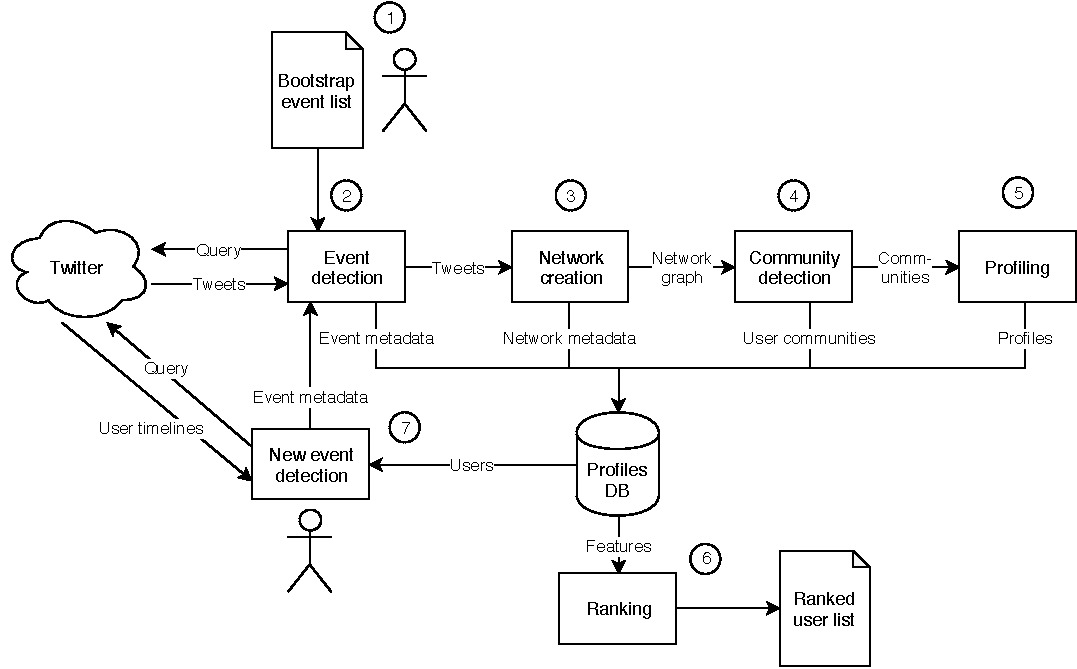
\includegraphics[width=0.7\linewidth]{figures/TwitterFramework}
	\caption{\comment{Schematic diagram of the user discovery framework }{this is a placeholder -- to be redrawn -PM }}
	\label{fig:twitterframework}
\end{figure*}

\subsection{Harvesting Content and Creating Context networks}  \label{sec:harvesting}

Firstly, all Twitter posts $P(C)$ that satisfy the criteria set in $C$ are retrieved, using either the Search or the Streaming Twitter APIs.\footnote{Repeat queries and multiple accouts are used to get around the well-known Twitter API limitations for retrieving tweets.}
%
Secondly, the context network $G_C$ is generated as defined in Sec.~\ref{sec:contexts}. To recall, this is a directed network representing retweet and/or mention interactions between pairs of users in $C$. 
The size of the network is largely determined by the nature of the context, and  ranges between 140 and 400 users (avg 254, see Table~\ref{tab:networks}).

\subsection{Community detection}  \label{sec:communities}

Next, the context network graph $G_C$  is partitioned into communities of users.
The goal of this partitioning is to further narrow the scope for the topology-sensitive metrics, namely FollowerRank (\ref{eq:FR}) and in-degree centrality (\ref{eq:IDC}), 
and thus to enable weak-signal users to emerge relative to other more globally dominant users.
%
Many different approaches have been proposed to discover virtual communities in social networks. 
We have chosen \demon~\cite{Coscia:2012:DLD:2339530.2339630} because it allows communities to overlap to a degree that is tunable, making it an ideal feature to identify users who may be active in more than one community within the same context, i.e., a social event or a campaign.

\demon identifies communities that a person belongs to with \textit{ego networks}, which consists of an individual, called the ego, and all the persons the ego has a social relationship with. 
As each ego network considers a node and its neighbours only, it provides a local method for discovering user affiliations, thus more akin to a social context.
%
It has been suggested~\cite{Arnaboldi2013} that ego networks are a useful model not only to describe social relationships amongst people offline, but also the structure of their online connections. 
Recognising that any individual may have different types of social relationships with different people (i.e., family, friends, colleagues, etc.),  \demon  naturally allows for an individual to participate in multiple communities. 

The locality principle of ego networks translates into an efficient algorithm for discovering overlapping communities in a social graph. 
Specifically, \demon operates on one node $v$ at a time in our context network $G_C$.

It applies a \textit{label propagation} algorithm to each neighbour $v'$ of $v$, as follows. First, a new label $l$, which identifies a new community, is tentatively assigned to $v'$. 
	Then, with probability $\alpha$ $v'$ changes its label to that of the majority of its own neighbours. 
	At this point, each of $v$'s neighbours has a label, which is either new of that of the majority of its own neighbours (excecpt $v$ itself).
	$v$ is then assigned majority labels amongst those of its neighbours. 
	This determines $v$'s community. 
	When more than one label has the same count, $v$ is assigned to all of those communities.
%
As a final step, communities that overlap by more than some percentage $\epsilon $ are merged.

Note that users who do not belong to any community are discarded from the whole process.
Once communities are identified, we calculate  in-degree centrality (\ref{eq:IDC}) for each node locally, \textit{relative to their own community}.

\comment{In our evaluation we have experimented with varying values for parameters $\alpha$ an $\epsilon$...}{do we plan to say anything on how to tune them?}

\anote{what happens when nodes belong to more than one community?}

\subsection{Computing user features and ranking  \anote{PM to fix wording}}  \label{sec:features}

The next step in the process involves retrieving the core features and then the user relevance metrics as defined in Sec. ~\ref{sec:metrics}, for each user in each of the communities.
%
As this involves querying the Twitter API for many user profiles, this step hits the limitations imposed by Twitter \anote{be specific}.
To get around this problem, we have implemented a dedicated component to \textit{scrape} user information directly from their profile Web pages, namely:
\begin{itemize}
	\item personal information: the name of the user, the link to its website, the bio and the date the user joined Twitter.
	\item profile statistics: the number of tweets published, and the number of followers $F1(u)$ as well as of followees, $F2(u)$.
\end{itemize}
The latter are used directly to compute  the \textit{Follower Rank} metric (\ref{eq:FR}).
To compute the other metrics: \textit{Topical Focus} (\ref{eq:TF}), \textit{Topical Strength} (\ref{eq:TS}), \textit{Topical Attachment} \ref{eq:TA}, we further need to retrieve the entire user post history for the entire time interval defined by the context.
These posts are then separated into $P(C)$ (on-context) and $\Tilde{P}(C)$ (off-context), depending on whether they contain a hashtag related to the context or not.
Similarly, a post that contains a link is a \textit{link on-topic} that contains both a link and an hashtag related to the context, and a \textit{link off-topic} otherwise.
Note that we also calculate the number of retweets for every post, i.e., $\mathit{R1}(u)$ and $\mathit{R3}(u)$, which are required to compute \textit{Topical Strength}.

All of these features are persisted to a database which is made available for ranking purposes.
When a user already appears in the database, i.e., from previous iterations, a user-defined function can be specified to update the set of features. 
For instance, one such function could just store the average over multiple occurrences of the same user across iterations, of each of the features as well as of the metrics.
Alternatively, the database allows for the series of features values to be stored, making it possible to analyse them over time.

The main purpose of the database is to enable data analytics on a growing set of users, whose history of engagement may extend over multiple events or campaigns.
In particular, ranking is achieved by specifying a user-defined function, as described in Fig.~\ref{fig:twitterframework}, which is a function of the metrics and generates a relevance score for each user.
Note that this ``framework'' approach is consistent with the experimental nature of our search for \textit{activists}, which requires exploring a variety of ranking functions.

\subsection{Context discovery} \label{sec:context-discovery}

The final step in the iteration aims to discover new contexts. 
The idea is that, once a score function has been applied and users have been ranked, we can hope to discover new interesting keywords and hashtags in the timeline of the top-$k$ users.
Specifically,  we consider each hashtag found in the timelines, which is related to the broader topic and not yet considered in past iterations.
Each stored hashtag is then enriched with the information needed to perform a new iteration of the pipeline, namely (i) the temporal and spatial information of the context, and (ii) related hashtags.

Currently this step is only semi-automated, as it requires a human to make a judgement on the relevance of the new terms. 
One can easily imagine this step to completely automated, however, and this is one of the items for our current work.

While the process ends naturally when no new contexts are uncovered from the previous ones, the system continuously monitors the Twitter stream for recent contexts. These may typically include events that are temporally recurring, and use similar hashtags for each new edition. In this case, their relevance is assessed on the basis of their past history.


\section{Empirical Evaluation} \label{sec:evaluation}

The typical approach to identifying specific classes on online users relies on expert-generated ground truth, i.e., to determine which users belong to the desired class. 
Such approach, however, is vulnerable to  the subjectivity of the experts, whereby the evalution would  be measuring the fit of the model to the specific experts' own opinion. 
In contrast, we follow an \textit{unsupervised} approach where there is no a priori knowledge of user relevance.  
We aim to demonstrate the value of our pipeline in creating a database of online profiles, pre-selected according to specific topological properties in order to filter out background noise,  along with a community-accepted set of engineered features that are ready to be mined using any user-defined function.

Thus, our evaluation (i) shows the pipeline in action on a significant set of contexts, and (ii) demonstrates useful ranking functions that operate on the resulting database.
Specifically, we  start by manually selecting homogeneous contexts from a single social domain, namely public healthcare campaigns, to demonstrate network construction, breakdown of each  context network into communities, and harvesting of users from each community, along with their metrics.
We then provide examples of ranking functions aimed at capturing the notion of  \textit{online activists}, and we empirically validate them by inspecting the profiles of representative top-k users.

 \subsection{Contexts and networks}  \label{sec:contexts}
 
 We have manually selected 25 contexts within the scope of health awareness campaigns in the UK, all occurring in 2018, all well-characterised using predefined hashtags.
 Table~\ref{tab:contexts}) lists the events along with key metrics for their corresponding user-user networks. 
To recall, \textit{assortativity} measures how frequently nodes are likely to connect to other nodes with the same degree (>0) or with a different degree (<0). 
Negative figures (mean: -0.22, std dev: 0.17) are in line with what is observed on the broader Twitter network \hl{add ref-about-assortativity-in-Twitter}.
%
The very small figures for density (mean: 0.004, std dev: 0.002), defined as $\frac{\#edges }{\mathit{\mathit{\#nodes}} (\mathit{\#nodes} -1)}$, suggest very few connections exist amongst users within a context. 
This makes it difficult to detect meaningful communities, as described below, thus for some context the topological metrics are measured on the entire network as opposed to within each community.
This view is also supported by the average node degree (mean: 2.04, std dev: 0.46) and the ratio of strongly connected components to the number of nodes (mean: 0.98, std. dev. 0.02).

\begin{table}
	
	\anote{content for this comes from cell [5] and cell [6] table 2 and cell [8]}
	
	\resizebox{\textwidth}{!}{%
		\begin{tabular}{|c|c|c|c|c|c|c|c|c|c|c|}
			\hline 
			\rule[-1ex]{0pt}{2.5ex} \textbf{Context name} &  \textbf{start date} & \textbf{end date}  & \textbf{hashtags} & \textbf{assortativity} & \textbf{avg degree} & \textbf{density} & \textbf{edges} & \textbf{nodes} & \textbf{scc / nodes} & \textbf{communities / nodes} \\ 
			\hline 
			\rule[-1ex]{0pt}{2.5ex} 16-days-of-action-2018  &  11-25&	12-10	& 	[\#16days, \#16daysofaction, \#16daysofactiontool...] & -0.1319 &  1.7626	 &  0.0022	 & 349 & 396 &  0.99 & 0\\ 
			\hline 
			\rule[-1ex]{0pt}{2.5ex}  elf-day &	12-03	& 12-12	&	[\#elfday, \#elfday2018] &  -0.1822	 &  2.3890	 & 0.0033	& 436	& 365	& 0.98  & 0.125 \\ 
			\hline 
			\rule[-1ex]{0pt}{2.5ex}  dry-january-2018	& 01-01	& 01-31	&	[\#dryjanuary] & -0.2833	 &  1.9915	& 0.0043	& 234	& 235	& 0.982979 & 0.25 \\ 
			\hline 
			\rule[-1ex]{0pt}{2.5ex}  cervical-cancer-prevention-week-2018	& 01-21	& 01-27	& 	[\#cervicalcancer]&  -0.0909	 &  1.8373	& 0.0044	& 192	& 209	& 0.976077 & 0.18 \\ 
			\hline 
			\rule[-1ex]{0pt}{2.5ex}  time-to-talk-day-2018	& 02-06	& 02-07	& [\#timetotalk]&  -0.2489	 &  1.7239	& 0.0032	& 231	& 268	& 0.988806 & 0.2 \\
			\hline 
			\rule[-1ex]{0pt}{2.5ex}  eating-disorder-awareness-week-2018	& 02-25	& 03-03	&	[\#edaw18, \#edaw2018, \#eatingdisordersawareness...]  &  -0.1544 & 1.8828	& 0.0037	& 241	& 256 & 0.988281 & 0.25 \\
			\hline 
			\rule[-1ex]{0pt}{2.5ex}  rare-disease-day-2018	& 02-28	& 03-01	& 	[\#rarediseaseday]&  -0.2443	 & 1.4014 & 0.0024	& 206	& 294 & 1.000000 & 0\\
			\hline 
			\rule[-1ex]{0pt}{2.5ex}  ovarian-cancer-awareness-month-2018	& 03-01	& 03-31	& 	[\#ovariancancer, \#ovariancancerawareness]  &  -0.3707	 & 1.8791	& 0.0044	& 202	& 215	& 0.986047 & 0\\
			\hline 
			\rule[-1ex]{0pt}{2.5ex}  nutrition-and-hydration-week-2018	& 03-11	& 03-17	&	[\#nutritionandhydrationweek, \#NHW2018]&  -0.2841	 &  2.3883	& 0.0044	& 326	& 273	& 0.985348 & 0.12\\
			\hline 
			\rule[-1ex]{0pt}{2.5ex}  brain-awareness-week-2018	& 03-11	03-17	& 2018-03-17 &	[\#brainawarenessweek, \#brainweek]& -0.0818	 &  1.8306	& 1.9349	& 281	& 307	& 0.996743 & 0 \\
			\hline 
			\rule[-1ex]{0pt}{2.5ex}  &  &  &  &  & & & & & & \\ 
			\hline 
	\end{tabular}}
	
	\anote{add the rest of the  data from the original tables}
	\caption{List of contexts used in the experiments along with network metrics and count of \demon communities}
	\label{tab:contexts}
\end{table}	 


\subsection{Communities}  \label{sec:communities}

Next, we report on the effect of the two community detection algorithms mentioned earlier, namely \demon and \hl{\textit{Girwan-Newman}}, on each of the networks. 
As we can see, within each network \demon either identifies a very small number of small communities, where it only retains users who belong to at least one community, or it ``disintegrates'' the network into degenerate, one-node communities. 
One-node communities are ignored by the pipeline. Whenever a network is broken down into one-node communities, the whole network is considered in users' in-degree calculations.
The rightmost column in Table~\ref{tab:contexts} reports the ratio of the number of communities to number of nodes in each of the networks.

Overall, \demon finds meaningful communities in 48\% of the networks, with 1.92 communities per network on average. 
As mentioned, when communities are meaningful, only users who belong to at least one community are added to the database. 
On average, for these networks this is 6\% of users.
In terms of connectedness and assortativity, unsurprisingly individual \demon communities are in line with the average for their parent networks, i.e., slightly negative average assortativity (details omitted due to space constraints).

%   cell [9]  not to be used

\anote{cell [10]: think about how to comment on histogram or omit altogether}

\anote{add report on Girwan-Newman communities }

\subsection{Users discovery}  \label{sec:users}

Finally, from each context we have extracted users who are either part of a community, or in the case of non-meaningful communities, all users in the network.
Using these criteria, a total of 3576 users has been added to the database from 25 contexts.
We are interested in tracking users' presence across more than one context, and in the specification of ranking functions that let specific user profiles emerge.

Regarding user presence, we found that there are 160 users who appear at least in two contexts. 
After community detection, only a fraction of these users survive. 
These are either users who belong to a meaningful community, or users who belong to a context network where communities could not be identified.

This filtering process results in 45 of the 160 users still seen as repeat users, while the remaining 115 are either removed altogether, or they only appear once. 
Out of these, 41 appear twice, and 4 appear three times. 
Thus, only 1.2\% of users appear more than once when communities are considered, compared to the overall 4.5\% repeat users.
%
Table~\ref{tab:repeat-users} reports the top repeat users along with their \textit{Follower Rank}.  \anote{comment on whether these are individuals or well-known organisations}
\anote{can we sort these by no-participation and follower-rank??}
%
Fig.~\ref{fig:repeat-users-frequency} shows the number of repeat users per context. 


\begin{table}
	\centering
	\framebox{\anote{content from cell [13]} }
	
	
	\caption{Top-k repeat users, amongst those identified as belonging to some community.}
	
	\label{tab:repeat-users}
\end{table}	 


\begin{figure*}
	\centering
	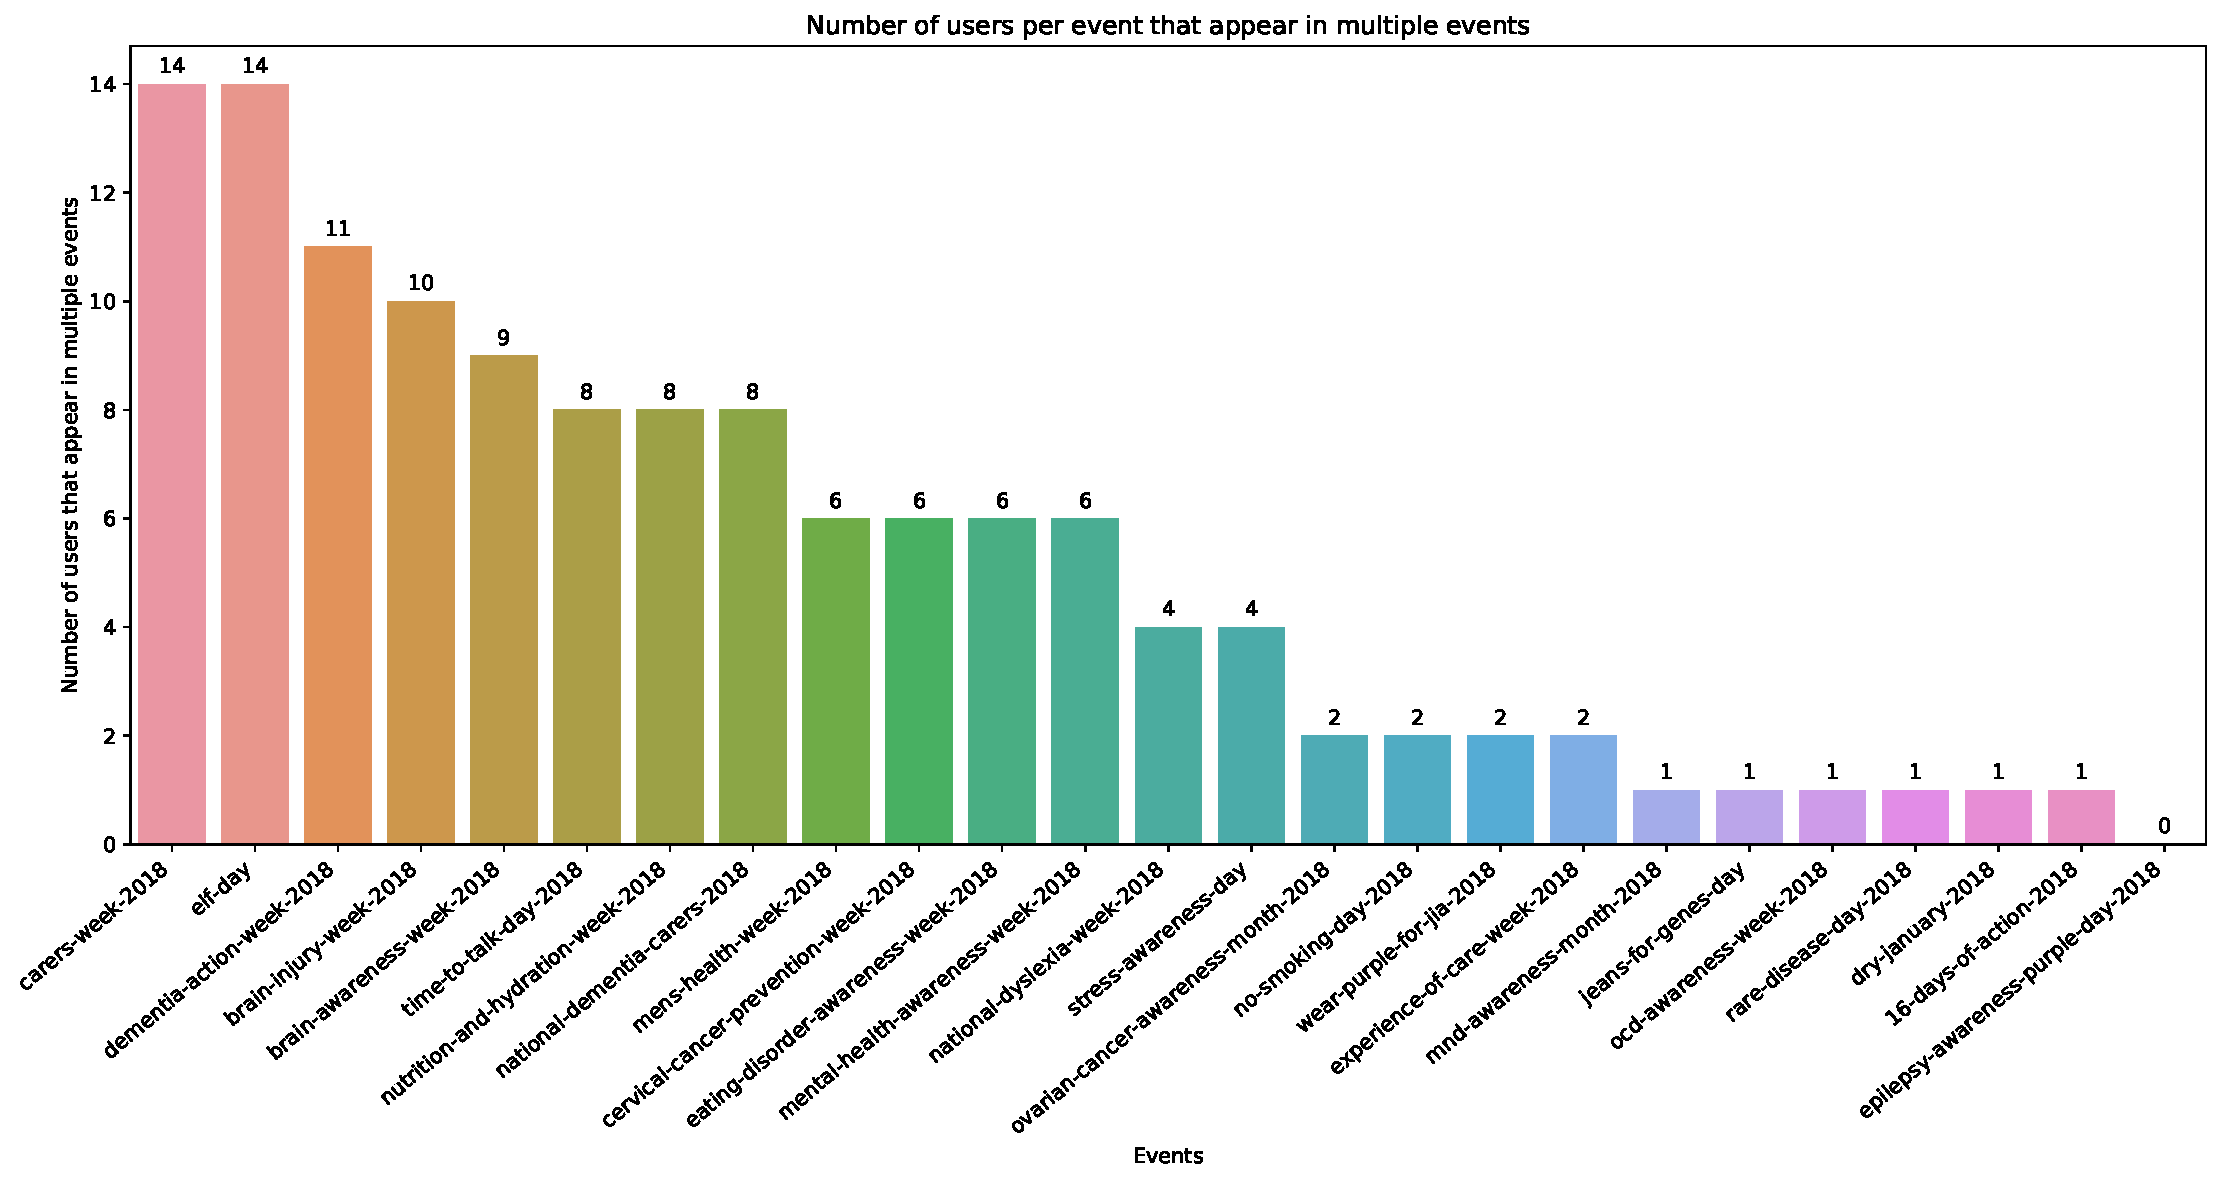
\includegraphics[width=1\linewidth]{figures/repeat-users-frequency}
	\caption{Number of repeat users for each context}
	\label{fig:repeat-users-frequency}
\end{figure*}

  \subsection{Users ranking} \label{sec:ranking}
  
  \anote{show the effect of one or two ranking functions and single out users that ``look like activists'' top empirically prove the point}
	
\section{Discussion and ongoing work}

\anote{
	we say that events are manually identified. Sketch the events bootstrapping idea.
}

\anote{FLAVIO:
	\begin{itemize}
		\item unsupervised learning?
	\end{itemize}
}

 \bibliographystyle{splncs04}
 \bibliography{icwe19}

\end{document}


\end{document}
